%% Beginning of file 'SN\,2020jgb.tex'
%% using aastex version 6.3
\documentclass[twocolumn]{aastex631}

\newcommand{\sn}{SN\,2020jgb}
\newcommand{\trmax}{$t_{r_\mathrm{ZTF},\mathrm{max}}$}
\newcommand{\tfl}{$t_\mathrm{fl}$}
\newcommand{\Mch}{$M_\mathrm{Ch}$}
\newcommand{\kms}{$\mathrm{km}\,\mathrm{s}^{-1}$}
\newcommand{\adam}[1]{\textcolor{red}{[AAM: #1]}}
\newcommand{\chang}[1]{\textcolor{blue}{[Chang: #1]}}

\shorttitle{\sn}
\shortauthors{Liu et al.}
\graphicspath{{./}{figures/}}

\begin{document}

\title{\sn: A Peculiar Type Ia Supernova Triggered by a Massive Helium-shell Detonation in a Star-forming Galaxy}

%main contributors
\author[0000-0002-7866-4531]{Chang~Liu}
\affiliation{Center for Interdisciplinary Exploration and Research in Astrophysics (CIERA), Department of Physics and Astronomy, Northwestern University, 1800 Sherman Road, Evanston, IL 60201, USA}

\author[0000-0001-9515-478X]{Adam~A.~Miller}
\affiliation{Center for Interdisciplinary Exploration and Research in Astrophysics (CIERA), Department of Physics and Astronomy, Northwestern University, 1800 Sherman Road, Evanston, IL 60201, USA}

\author[0000-0002-2028-9329]{Anya~E.~Nugent}
\affiliation{Center for Interdisciplinary Exploration and Research in Astrophysics (CIERA), Department of Physics and Astronomy, Northwestern University, 1800 Sherman Road, Evanston, IL 60201, USA}

\author[0000-0002-2028-9329]{Abigail~Polin}
\affiliation{The Observatories of the Carnegie Institution for Science, 813 Santa Barbara Street, Pasadena, CA 91101, USA}
\affiliation{TAPIR, Walter Burke Institute for Theoretical Physics, 350-17, Caltech, Pasadena, CA 91125, USA}

%spectra
\author[0000-0002-8977-1498]{Igor~Andreoni}
\altaffiliation{Neil Gehrels Fellow}
\affil{Joint Space-Science Institute, University of Maryland, College Park, MD 20742, USA.}
\affil{Department of Astronomy, University of Maryland, College Park, MD 20742, USA.}
\affil{Astrophysics Science Division, NASA Goddard Space Flight Center, Mail Code 661, Greenbelt, MD 20771, USA}

\author[0000-0001-5955-2502]{Thomas~G.~Brink}
\affiliation{Department of Astronomy, University of California, Berkeley, CA 94720-3411, USA}

\author[0000-0003-3460-0103]{Alexei V. Filippenko}
\affiliation{Department of Astronomy, University of California, Berkeley, CA 94720-3411, USA}

%\author{Tassilo~Schweyer}
%\affiliation{The Oskar Klein Centre, Department of Astronomy, Stockholm University, AlbaNova, SE-106 91 Stockholm, Sweden}

%builders
\author[0000-0001-5668-3507]{Steven~L.~Groom}
\affiliation{IPAC, California Institute of Technology, 1200 E. California Blvd, Pasadena, CA 91125, USA}

\author{David~Hale}
\affiliation{Caltech Optical Observatories, California Institute of Technology, Pasadena, CA 91125, USA}

\author[0000-0002-8532-9395]{Frank~J.~Masci}
\affiliation{IPAC, California Institute of Technology, 1200 E. California Blvd, Pasadena, CA 91125, USA}

\author[0000-0003-1227-3738]{Josiah~Purdum}
\affiliation{Caltech Optical Observatories, California Institute of Technology, Pasadena, CA 91125, USA}

\author[0000-0001-8861-3052]{Benjamin~Racine}
\affiliation{Aix Marseille Univ, CNRS/IN2P3, CPPM, Marseille, France}

\author[0000-0003-1546-6615]{Jesper~Sollerman}
\affiliation{The Oskar Klein Centre, Department of Astronomy, Stockholm University, AlbaNova, SE-106 91 Stockholm, Sweden}

\author[0000-0001-5390-8563]{Shrinivas~R.~Kulkarni}
\affiliation{Department of Astronomy, California Institute of Technology, 1200 E. California Blvd, Pasadena, CA, 91125, USA}

\author{Other fantastic astronomers}

\begin{abstract} 
%
The detonation of a thin ($\lesssim$0.03\,$\mathrm{M_\odot}$) helium shell (He-shell) atop a white dwarf (WD) is a promising mechanism to explain normal Type Ia supernovae (SNe\,Ia), while thicker He-shells ($>$0.03\,$\mathrm{M_\odot}$) may explain some recently observed peculiar SNe\,Ia. We present observations of \sn, a peculiar SN\,Ia discovered by the Zwicky Transient Facility (ZTF). Near maximum light, \sn\ is sub-luminous (ZTF $g$-band absolute magnitude $M_g\approx -18.2$\,mag) and shows an unusually red color ($g_\mathrm{ZTF}-r_\mathrm{ZTF}\approx 0.4$\,mag) due to the strong line-blanketing bluewards of $\sim$5000\,\AA. These properties resemble SN\,2018byg, a peculiar SN\,Ia resulting from a ``thick He-shell'' double detonation (DDet). Using detailed radiative transfer models, we show that the optical spectroscopic and photometric evolution of \sn\ are broadly consistent with a He-shell of $\sim$0.08\,$\mathrm{M_\odot}$ detonating above a carbon-oxygen WD of $\sim$0.87\,$\mathrm{M_\odot}$. We detect a prominent absorption feature at $\sim$1\,\micron\ in the near-infrared (NIR) spectrum of \sn, which could originate from the unburnt helium in the outermost ejecta. While the sample size is limited, similar 1\,\micron\ features have been detected in all the thick He-shell DDet candidates with NIR spectra obtained to date. \sn\ is also the first thick He-shell DDet SN discovered in a star-forming galaxy, indisputably showing that He-shell DDet objects occur in both star-forming and passive environments, consistent with the normal SN\,Ia population.
%
\end{abstract}

\keywords{Supernovae(1668), Type Ia supernovae(1728), White dwarf stars(1799), Observational astronomy(1145), Surveys(1671)}

\section{Introduction} \label{sec:intro}
It has been clear for decades that Type Ia supernovae (SNe\,Ia) are caused by the thermonuclear explosions in carbon-oxygen (C/O) white dwarfs (WDs) in binary systems \citep[see][for a review]{Maoz_2014}. Nevertheless, the nature of the binary companion, as well as how it ignites the WD, remains highly uncertain. 

The helium-shell (He-shell) double detonation (DDet) scenario is one of the most promising channels to produce SNe\,Ia. In this scenario, the WD accretes from a companion to develop a helium-rich shell, which, once becomes massive enough, could detonate. Such a detonation sends a shock wave into the C/O core to trigger a runaway thermonuclear explosion and inevitably disrupts and destroys the entire WD \citep{Nomoto_1982a, Nomoto_1982b, Woosley_1986, Livne_1990, Woosley_1994, Livne_1995}. This DDet mechanism can produce explosions in WDs below the Chandrasekhar-mass (\Mch).

There are several observational benchmarks for He-shell DDet triggered SNe. Shortly after the ignition of He-shell, the decay of radioactive material in the helium ashes may power a detectable flash \citep{Woosley_1994,Fink_DD_2010,Kromer_DD_2010}. The Fe-group elements in the ashes will blanket blue photons with wavelengths $\lesssim$5000\,\AA\ \citep{Kromer_DD_2010}, the duration of which depends on the mass of the He-shell. For thick enough shells, \citet{Boyle2017_Helium} suggest that the unburnt helium could provide an observational signal in NIR spectra, and \citet{polin_nebular_2021} predict significant [\ion{Ca}{2}] emission in the nebular phase of the SNe.

Using different sets of He-shell mass and C/O core mass, one can reproduce a variety of observables in `normal' SNe\,Ia with typical luminosities and spectral features near peak light \citep[e.g.,][]{polin_observational_2019,Shen_2D_2021}, or peculiar sub-luminous ones \citep[e.g.,][]{polin_observational_2019}. 

For the DDet SNe that show `normal' characteristics near their peaks, the mass of the He-shell is expected to be low \citep[$\lesssim$0.03\,$\mathrm{M_\odot}$;][]{Kromer_DD_2010,Sim_2010,Shen_DD_2018,polin_observational_2019}. The first reported He-shell DDet candidate with a thin He-shell was SN\,2016jhr \citep{jiang_16jhr_2017}, which exhibits an early red flash and keeps a red $g-r$ color throughout its evolution, though it shows a typical absolute magnitude at peak ($M_g\approx-19$) for normal SNe\,Ia. The multi-band light curves involving the early flash and the major peak, as well as the optical spectrum close to the peak light, could be simultaneously fit by a near-\Mch\ DDet model (a 1.38\,$\mathrm{M_\odot}$ C/O core and a 0.03\,$\mathrm{M_\odot}$ He-shell). Recently, it was reported that SN\,2018aoz \citep{Ni_2022}, a SN\,Ia showing a rapid redward color evolution within $\sim$12\,hr after the first light, could be explained by a sub-\Mch\ DDet model (a 1.05\,$\mathrm{M_\odot}$ C/O core and a 0.03\,$\mathrm{M_\odot}$ He-shell). After this red excess the photometric evolution is consistent with normal SNe\,Ia, when the ashes of the thin He-shell become optically thin. However, some of its peak-time and nebular phase spectral properties are not consistent with a He-shell DDet scenario \citep{Ni_2022b}, making its nature debatable. To date, only a small fraction of SNe\,Ia have been discovered early enough for possible detection of early flashes \citep[e.g.,][]{Deckers_2022}. While there could be a large underlying population of normal SNe\,Ia triggered by He-shell DDet, currently it is hard to verify this scenario.

In contrast, if the He-shell mass is much greater than 0.03\,$\,\mathrm{M_\odot}$, the ashes of the He-shell detonation could remain optically thick over a much more extended time, resulting in the red color and low luminosity near peak light. SN\,2018byg \citep{de_18byg_2019} is a prototype of thick He-shell DDet SNe. During the late stages of preparing for this paper, \citet{Dong_16dsg_2022} presented another thick He-shell DDet candidate, SN\,2016dsg, accompanied with an archival transient OGLE-2013-SN-079 \citep{Inserra_OGLE13_079_2015}. All three candidates are faint, red, and show strong line-blanketing in maximum-light spectra. A tentative detection of unburnt helium in SN\,2016dsg was also reported in \citet{Dong_16dsg_2022}. The small sample size to date suggests thick He-shell events might be intrinsically rare.

It has been suggested that some, if not all, of the calcium-rich (Ca-rich) gap transients, a population of faint SNe with conspicuous [\ion{Ca}{2}] emission in the nebular phase, also arise from He-shell DDet \citep{Dessart_2015,de_Ca_rich_2020,polin_nebular_2021}. A subclass of Ca-rich transients resemble SNe\,Ia near peak light (termed Ca-Ia objects), marked by the strong \ion{Si}{2} absorption and the absence of optical \ion{He}{1} lines. There are only three Ca-Ia objects \citep[PTF\,09dav, SN\,2016hnk, and SN\,2019ofm;][]{de_Ca_rich_2020}, all showing mild to strong line-blanketing in spectra, and hence could be He-shell DDet objects \citep[e.g.,][]{jacobson-galan_16hnk_2020}. Nonetheless, they also exhibit properties similar to other types of sub-luminous SNe\,Ia, such as the strong \ion{O}{1} absorption widely seen in 91bg-like objects \citep{Filippenko_91bg_1992} but not prominent in other He-shell DDet candidates. PTF\,09dav shows the weakest line-blanketing among the three and exhibits features that are attributed to some rare elements such as \ion{Sc}{2} \citep{Sullivan_2011}, which cannot be immediately explained by either He-shell DDet or deflagration models. SN\,2016hnk could also be explained by the deflagration of a near-\Mch\ WD \citep{galbany_16hnk_2019}. In summary, the nature of Ca-Ia objects remains ambiguous.

In this paper, we present the observations of another promising thick He-shell DDet candidate, \sn. This peculiar SN\,Ia highly resembles SN\,2018byg in photometric and spectroscopic properties, and exhibits a remarkable feature in the NIR spectrum that could be attributed to the unburnt helium. In Section~\ref{sec:obs} we report the observations of \sn, which are analyzed in Section~\ref{sec:analysis}, where we show its similarities with other He-shell DDet SNe and discuss the tentative \ion{He}{1} absorption features. We use a grid of He-shell DDet models to fit the data of \sn, and present the results in Section~\ref{sec:model}. Then we expand our discussion to other He-shell DDet SNe, discussing the possibly ubiquitous absorption features in their NIR spectra near 1\,\micron\ (Section~\ref{sec:1um}) and their diversity in host environments (Section~\ref{sec:host}). We draw our conclusions in Section~\ref{sec:conclusion}.

\section{Observations} \label{sec:obs}
\subsection{Discovery}

\sn\ was first discovered by the Zwicky Transient Facility \citep[ZTF;][]{ZTF2019a,ZTF2019b} on 2020 May 03.463 UT (MJD 58972.463) with the 48-inch Samuel Oschin Telescope (P48) at Palomar Observatory. The automated ZTF discovery pipeline \citep{Masci_2019} detected \sn\ using the image-differencing technique of \citet{Zackay_imagesub_2016}. The candidate passed internal thresholds \citep[e.g.,][]{Mahabal_ZTFML_2019, Duev_ZTFML_2019}, leading to the production and dissemination of a real-time alert \citep{Patterson_ZTFalert_2019} and the internal designation ZTF20aayhacx. It was detected with $g_\mathrm{ZTF} = 19.86 \pm 0.15\,$mag at $\alpha_\mathrm{J2000}=17^\mathrm{h}53^\mathrm{m}12^\mathrm{s}.651$, $\delta_\mathrm{J2000}=-00^\circ51'21\farcs{81}$ and announced to the public in \citet{Fremling_report_2020}. The host galaxy, PSO J175312.663+005122.078, is a dwarf galaxy, to which \sn\ has a projected offset of only $0\farcs3$. The last non-detection limits the brightness to $r_\mathrm{ZTF} > 20.7$\,mag on 2020 April 27.477 (MJD 58966.477; 5.99\,days before the first detection). This transient was classified as a SN\,Ia in \citet{TNS_2020}.

\subsection{Host Galaxy Observations}
On 2022 March 31, two years after the transient faded, we took a spectrum for its host galaxy using the DEep Imaging Multi-Object Spectrograph (DEIMOS) on the Keck II telescope \citep{DEIMOS_2003}, with a total integration time of 3200\,s. It was reduced with the \texttt{PypeIt} Python package \citep{pypeit:joss_pub}. The reduced spectrum is displayed in Figure~\ref{fig:host_spec}. 
The host exhibits strong, narrow emission lines including H$\alpha$, H$\beta$, [\ion{N}{2}] $\lambda\lambda$6548, 6583, [\ion{O}{3}] $\lambda\lambda$4959, 5007, and [\ion{S}{2}] $\lambda\lambda$6716, 6731. By fitting all these emission features with Gaussian profiles we obtain an average redshift of $z=0.0309\pm0.0003$. With the diagnostic emission line equivalent width (EW) ratios ($\log$~[\ion{N}{2}]/H$\alpha=-1.19\pm0.07$ and $\log$~[\ion{O}{3}]/H$\beta=0.53\pm0.06$)\footnote{Here [\ion{N}{2}] denotes the EW of the [\ion{N}{2}] $\lambda$6583 line, and [\ion{O}{3}] denotes the EW of the [\ion{O}{3}] $\lambda$5007 line.}, the host is consistent with star-forming galaxies in the BPT diagram \citep{BPT_1981, Veilleux_1987}. 

To estimate the distance modulus to \sn, we first use the 2M++ model \citep{Carrick2015_2M++} to obtain the peculiar velocity towards its host galaxy, PSO\,J175312.663+005122.078, to be $179\pm250$\,\kms. This, combined with the recession velocity in the frame of the cosmic microwave background\footnote{\url{https://ned.ipac.caltech.edu/velocity_calculator}} (CMB) $v_\mathrm{CMB}=9136$\,\kms, yields a net Hubble recession velocity of $9307\pm250$\,\kms. Adopting $H_0=70$\,\kms\,Mpc$^{-1}$, $\Omega_M=0.3$, and $\Omega_\Lambda=0.7$, we estimate the luminosity distance to \sn\ to be 136.1\,Mpc, which yields a distance modulus of $\mu=35.66\pm0.06$\,mag.

\subsection{Optical Photometry}
\sn\ was monitored in the $g_\mathrm{ZTF}$ and $r_\mathrm{ZTF}$-bands by ZTF as part of its ongoing Northern Sky Survey \citep{Bellm_2019}. We adopt a Galactic extinction of $E(B-V)=0.404\,$mag \citep{Schlafly2011}, and correct all photometry using the \citet{Fitzpatrick1999} extinction model. We assume there is no additional extinction in the host galaxy. This assumption is supported by the lack of \ion{Na}{1} D absorption at the redshift of the host galaxy, though see \citet{Poznanski_2011} for caveats on the use of \ion{Na}{1} D absorption as a proxy for extinction. 

The forced photometry light curves\footnote{\url{https://web.ipac.caltech.edu/staff/fmasci/ztf/forcedphot.pdf}} in absolute magnitudes in $g_\mathrm{ZTF}$- and $r_\mathrm{ZTF}$-bands are shown in Figure~\ref{fig:photometry}, in which we show all the measurements with a siginal-to-noise ratio (SNR) greater than 2. The light curves are reduced using the pipeline from Miller et al. (2022, in preparation). See also \citet{Yao_2019}. %\chang{Should also add a citation to Yuhan's paper as a see also} %\chang{Should point to ZTF forced light curve service as a reference here - probably also make sense to cite Miller et al. in prep since I made the light curve}

\begin{figure*}
    \centering
    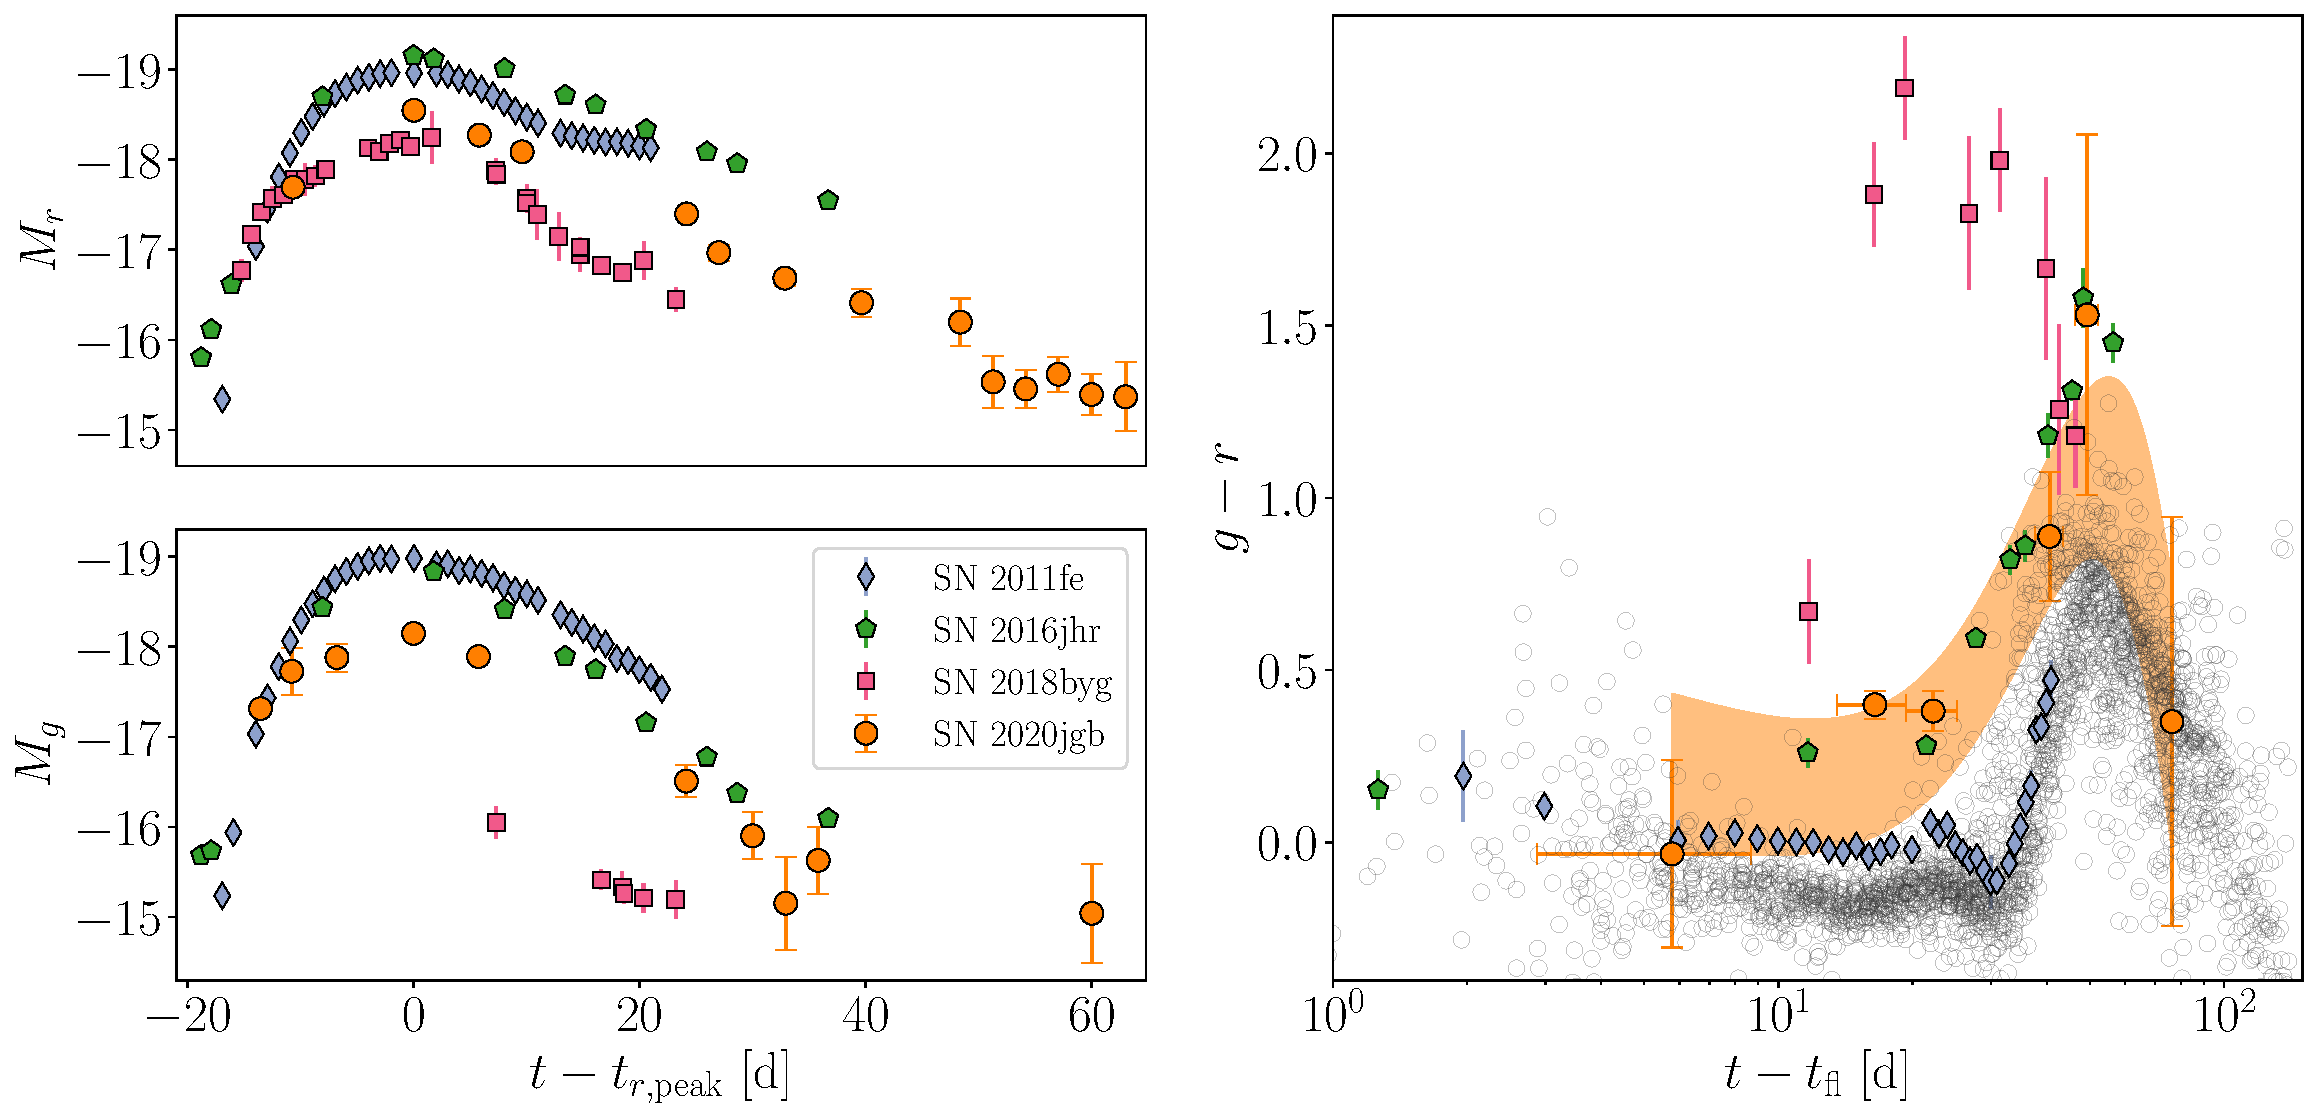
\includegraphics[width=\textwidth]{photometry.pdf}
    \caption{Comparison of the photometric properties of \sn\ with SN\,2011fe \citep[normal SN\,Ia;][]{Pereira_2013}, SN\,2016jhr \citep[normal-luminosity He-shell DDet;][]{jiang_16jhr_2017}, and SN\,2018byg \citep[sub-luminous He-shell DDet;][]{de_18byg_2019}. \textit{Left}: Multi-band light curves. The upper (lower) panel shows the evolution in $r$-band ($g$-band) absolute magnitudes. \textit{Right}: $g-r$ color evolution. The grey circles denote the $g_\mathrm{ZTF}-r_\mathrm{ZTF}$ color evolution of 62 normal SNe\,Ia (open circles) with prompt observations within 5\,days of first light by ZTF \citep{Bulla2020}.}
    \label{fig:photometry}
\end{figure*}

\subsection{Optical Spectroscopy}\label{sec:optical_spec}
We obtained optical spectroscopic follow-up of the object from $\sim$$-10$\,days to $\sim$$+150$\,days relative to the $r_\mathrm{ZTF}$-band peak, using the Spectral Energy Distribution Machine \citep[SEDM;][]{SEDM_2018} on the automated 60\,inch telescope \citep[P60;][]{P60_2006} at Palomar Observatory, the Kast Double Spectrograph \citep{miller1994kast} at the Shane 3\,m Telescope, the Andalucia Faint Object Spectrograph and Camera (ALFOSC)\footnote{\url{https://www.not.iac.es/instruments/alfosc/}} installed at the Nordic Optical Telescope (NOT), the Double Beam Spectrograph (DBSP) on the 200\,inch Hale telescope \citep[P200;][]{P200_1982}, the Low Resolution Imaging Spectrograph (LRIS) on the Keck I telescope \citep{Keck_1995}. With the exception observations obtained with SEDM, all spectra were reduced using standard procedures \citep[e.g.,][]{Matheson_2000}. The SEDM spectra were reduced using the custom \texttt{pysedm} software package \citep{Rigault_pysedm_2019}. Details of the spectroscopic observations are listed in Table~\ref{tab:spec}, and the spectral sequence is shown in Figure~\ref{fig:spec_evo}.

\begin{deluxetable}{lrcccc}
\tabletypesize{\scriptsize}
\tablewidth{0pt}
\tablecaption{Spectroscopic Observations of \sn\label{tab:spectra}}
\tablehead{
\colhead{$t_\mathrm{obs}$} &
\colhead{Phase} &
\colhead{Telescope/} &
\colhead{$R$} &
\colhead{Range} &
\colhead{Air} \\
\colhead{(MJD)} &
\colhead{(d)} &
\colhead{Instrument} &
\colhead{$(\lambda/\Delta\lambda)$} &
\colhead{(\AA)} & 
\colhead{Mass}
}
\startdata
58,976.42 &  $-$9.7 & P60/SEDM & 100 & 3770--9220 & 1.23\\
58,982.12 & $-$4.2 & NOT/ALFOSC & 360 & 4000--9620 & 1.17\\
58,990.43 &  $+$3.9 & P60/SEDM & 100 & 3770--9220 &  1.23\\
58,997.44 & $+$10.7 & P60/SEDM & 100 & 3770--9220 &  1.29\\
58,998.41 & $+$11.6 & Shane/Kast & 1000? & 3620--10720 & 1.28\\
59,008.41 & $+$21.3 & P60/SEDM & 100 & 3770--9220 & 1.28\\
59,010.40 & $+$23.3 & P200/DBSP & 700 & 3200--9500 &  1.27\\
59,023.58 & $+$36.1 & Keck I/LRIS & 1100 & 3200--10250 & 2.04\\
59,107.29 & $+$117.3 & Keck I/LRIS & 1100 & 3200--10250 & 1.31\\
59,143.26 & $+$152.2 & Keck I/LRIS & 1100 & 3200--10250 & 2.16\\
\enddata
\tablecomments{Phase is measured relative to \trpeak\ in the host galaxy rest frame. The resolution $R$ is reported for the central region of the spectrum.}
\end{deluxetable}
\begin{figure*}
    \centering
    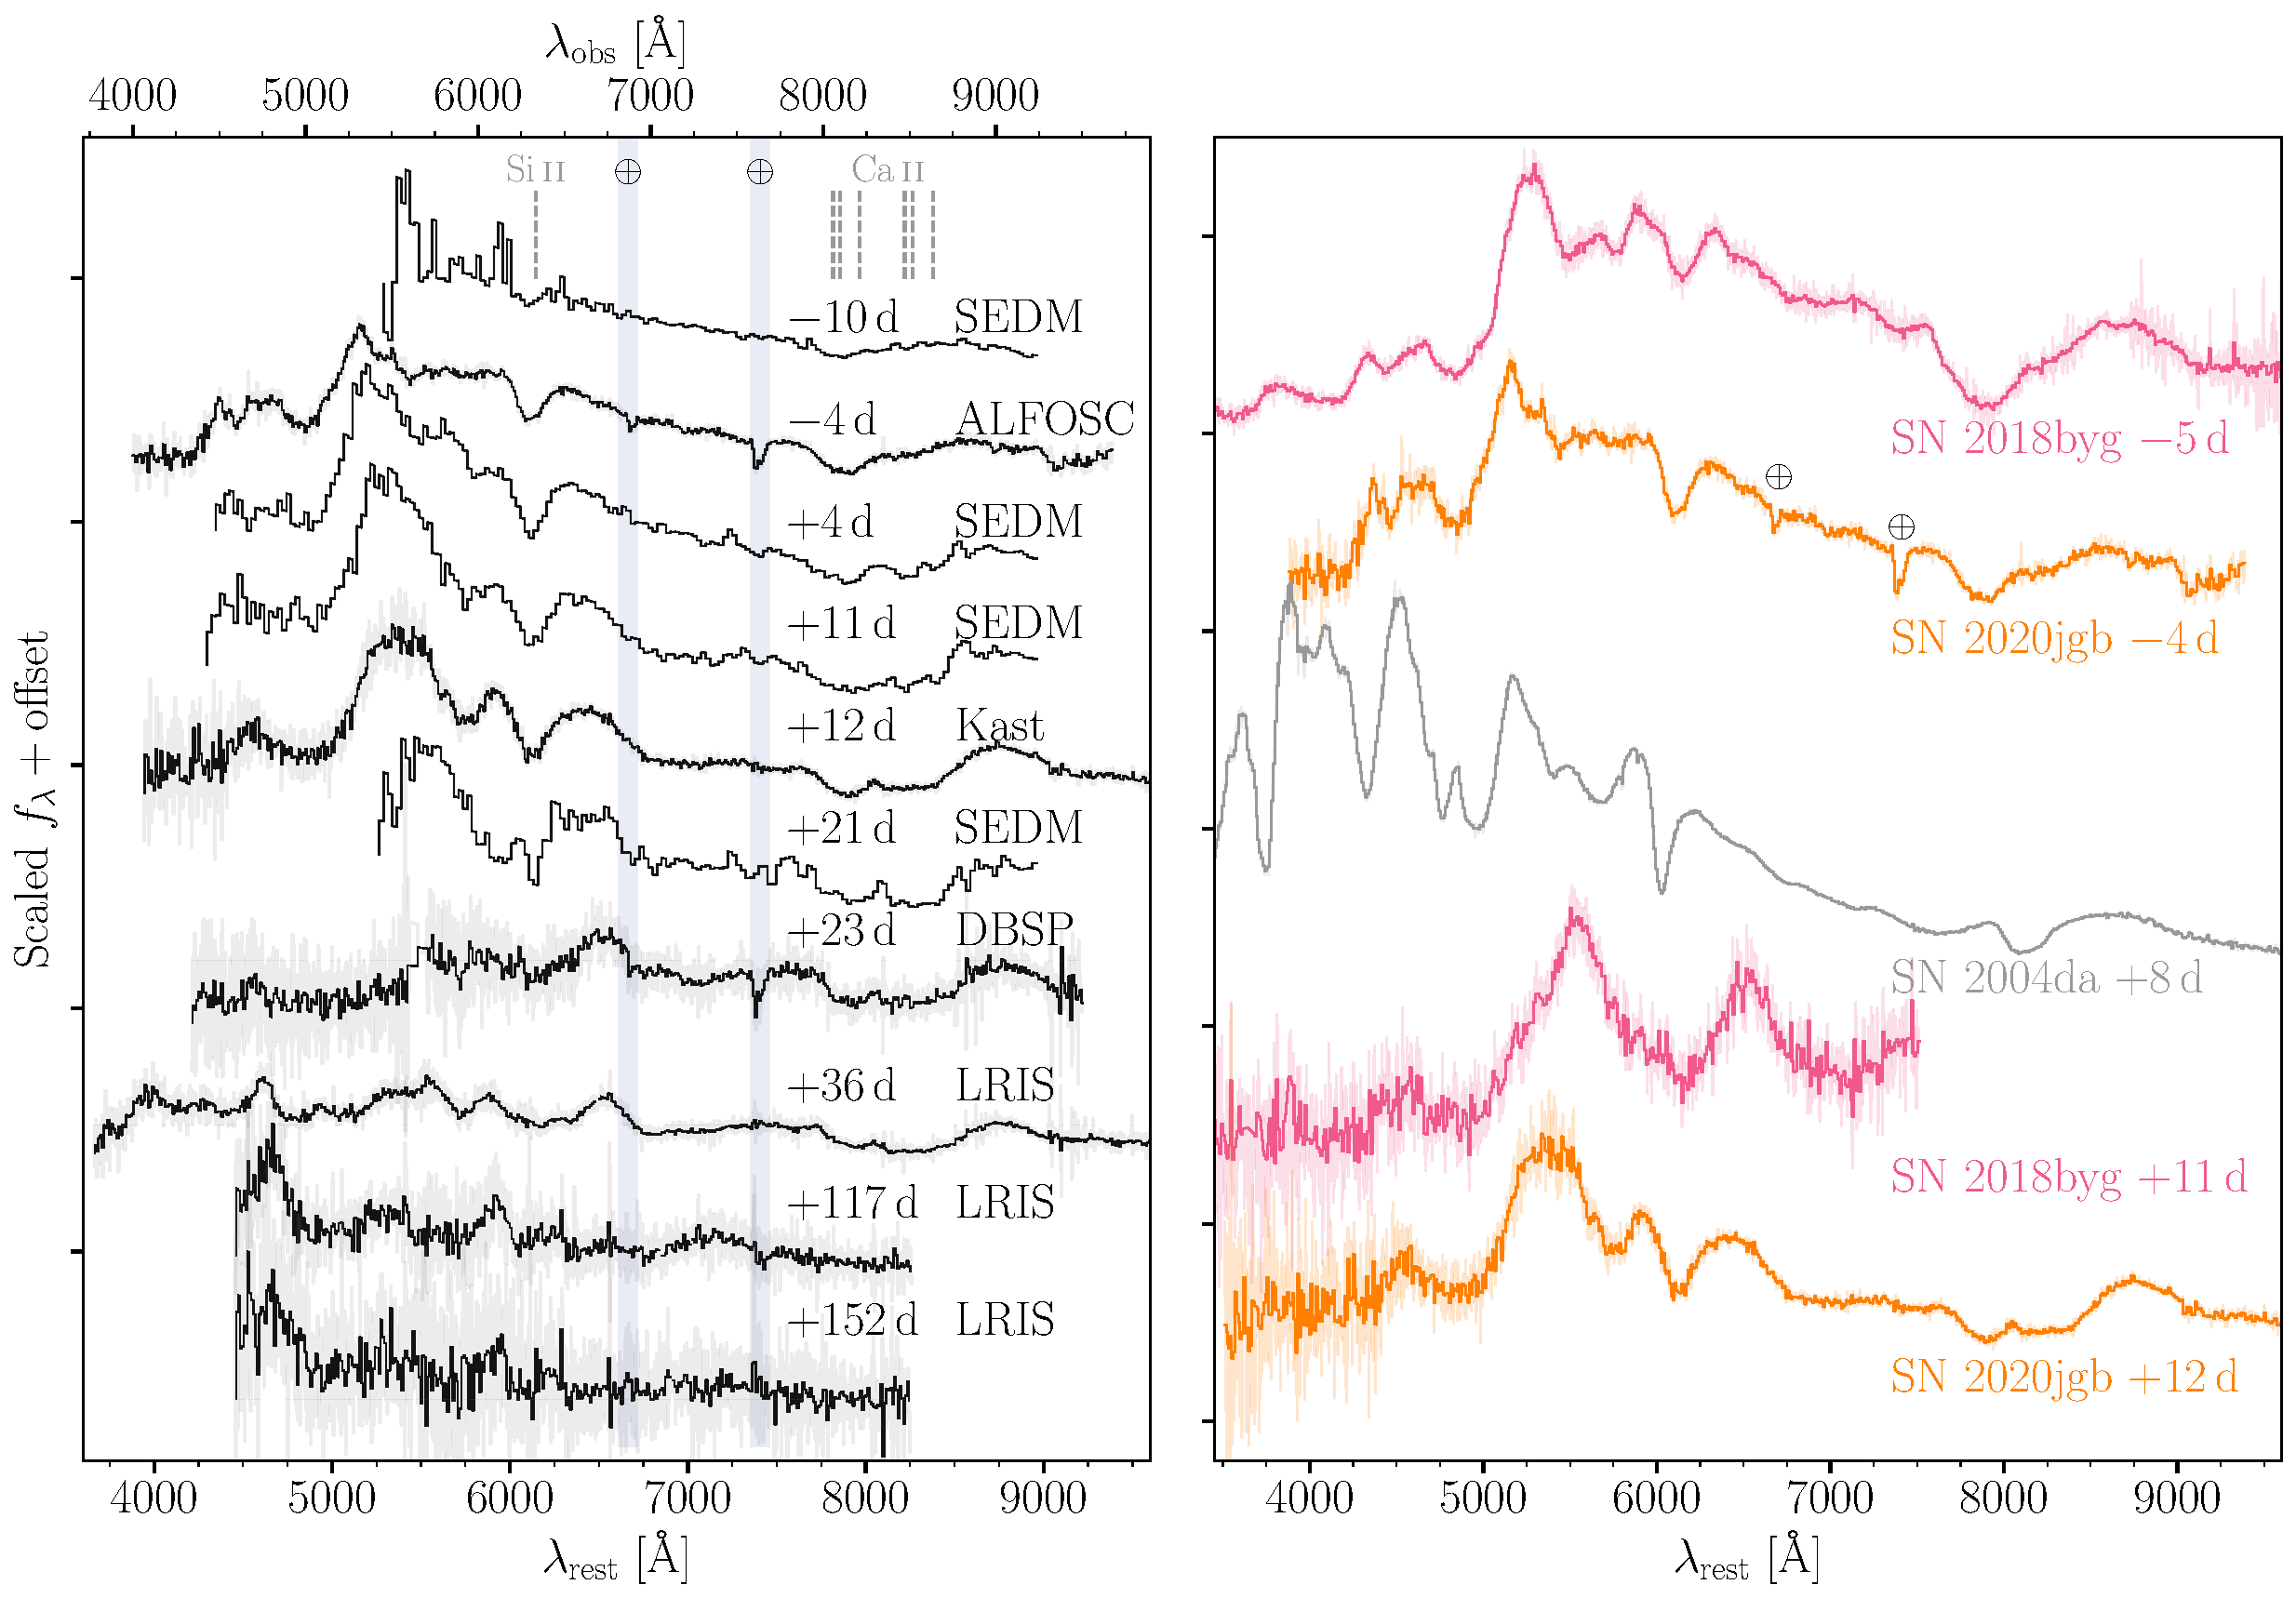
\includegraphics[width=\textwidth]{optical_spec_evolution.pdf}
    \caption{The optical spectra of \sn, typical for a peculiar SN Ia triggered by He-shell DDet. \textit{Left}: optical spectral sequence of \sn. Rest frame phases (days) relative to the $r_\mathrm{ZTF}$-band peak and instruments used are posted next to each spectrum. The spectra after Galactic extinction correction are shown in grey. The black lines are binned spectra with a bin size of 10\,\AA, except for the SEDM spectra, whose resolution is lower than the bin size. In the last two spectra, we have subtracted the light from the host galaxy. Only regions with $\mathrm{SNR}>2.5$ after binning are plotted. 
    \textit{Right}: spectral comparison with SN\,2018byg \citep[sub-luminous He-shell DDet;][]{de_18byg_2019} and SN\,2004da \citep[normal luminosity;][]{Silverman_2012}.}
    \label{fig:spec_evo}
\end{figure*}

\subsection{Near-infrared (NIR) Spectroscopy}
We obtained one NIR (0.8-2.5\,\micron) spectrum of \sn\ using the Gemini near-infrared spectrometer \citep[GNIRS;][]{GNIRS1998} on the Gemini North telescope on 2020 June 9 ($\sim$22\,days after $r_\mathrm{ZTF}$-band peak), with an integration time of 2400\,s. The GNIRS spectrum was reduced with \texttt{PypeIt}.

\begin{figure*}
    \centering
    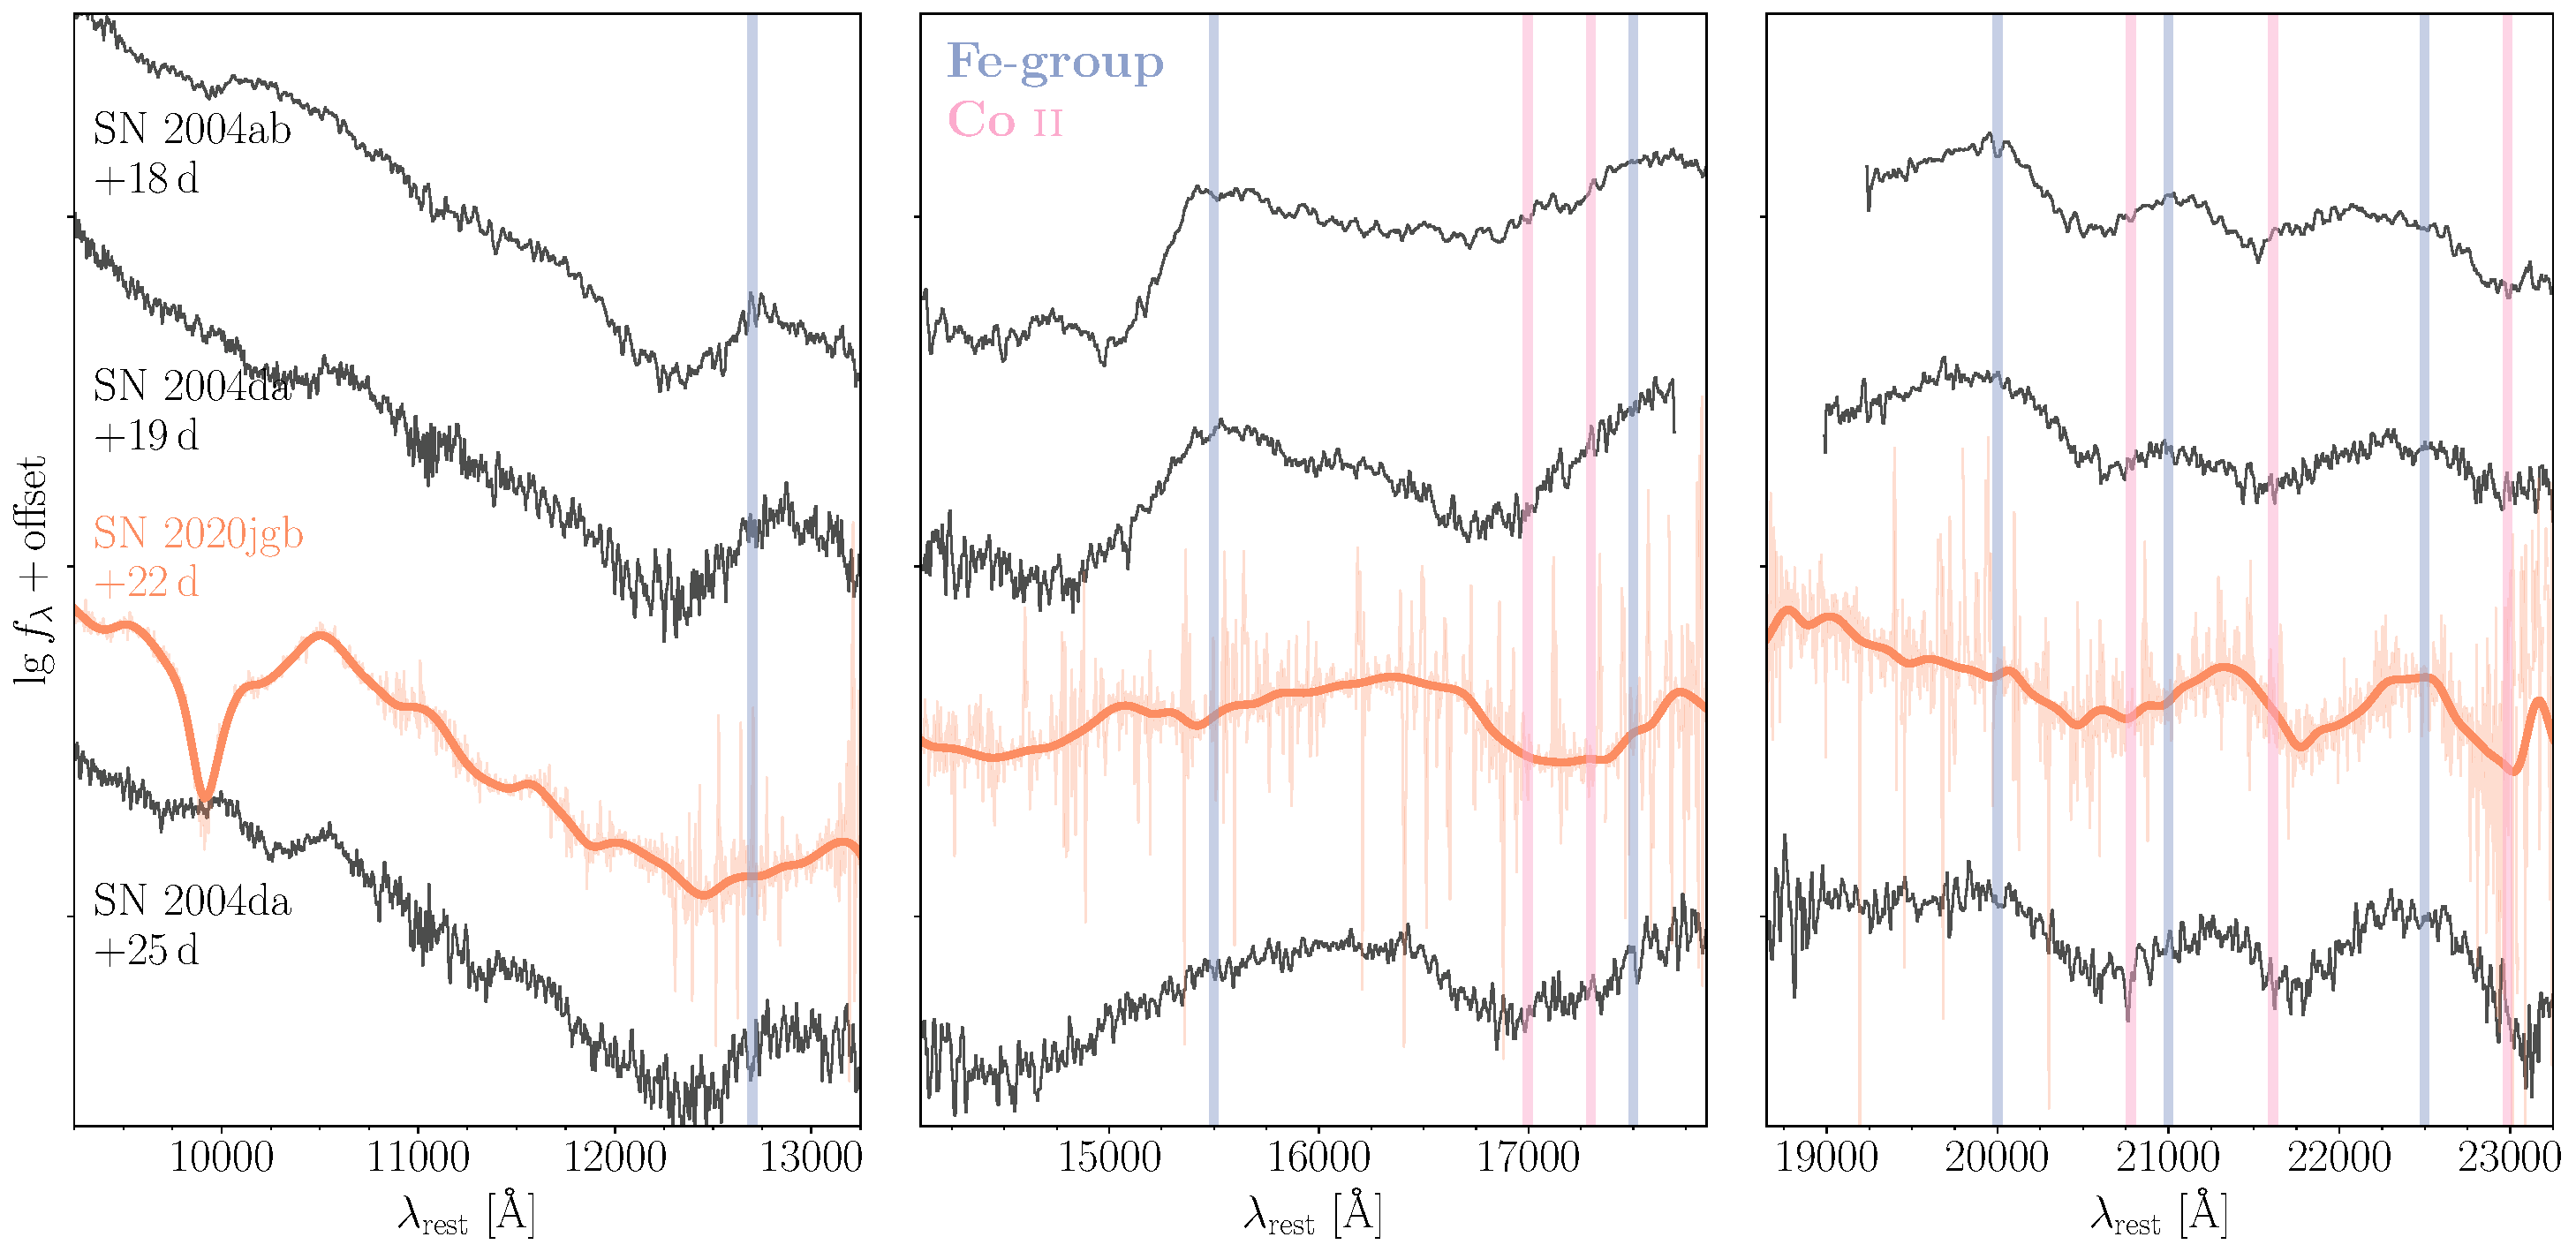
\includegraphics[width=\textwidth]{NIR_spec.pdf}
    \caption{The NIR spectra of \sn\ and two normal-luminosity SNe\,Ia, SN\,2004ab and SN\,2004da \citep{Marion2009_NIR}, both showing highly similar spectral features expect the absorption line near 1\,\micron. All spectra were obtained at similar phases. For each spectrum, the continuum at $\gtrsim$1.2\,\micron\ is significantly reshaped by the line-blanketing from Fe-group elements (blue vertical lines), which are continuous emission features composed of unresolved Fe-group lines peaking at $\sim$1.27, 1.55, 1.75, 2.00, 2.10, 2.25\,\micron\ \citep{Marion2009_NIR}. Between these peaks lie multiple strong \ion{Co}{2} absorption lines (pink vertical lines), for which a typical post-maximum expansion velocity of 8,000\,\kms is assumed. The grey vertical lines correspond to \ion{Fe}{2} $\lambda$9998 and \ion{Fe}{2} $\lambda$10500, also with an expansion velocity of 8,000\,\kms.}
    \label{fig:NIR_spec}
\end{figure*}

\section{Analysis} \label{sec:analysis}
\subsection{Photometric Properties}
\sn\ exhibited a fainter light curve than normal SNe\,Ia. In Figure~\ref{fig:photometry}, we compare the photometric properties of \sn\ with the nearby, well-observed SN\,2011fe with ZTF $g$- and $r$-band synthetic photometry from the spectrophotometric time series in \citet{Pereira_2013}, as well as two He-shell DDet candidates, including the normal-luminosity thin shell candidate SN\,2016jhr \citep{jiang_16jhr_2017} and the sub-luminous thick He-shell candidate SN\,2018byg \citep{de_18byg_2019}. All these light curves have been corrected for Galactic reddening, while $K$-corrections have not been performed\footnote{These SNe were all observed in slightly different $g$- and $r$-filters.}.

While the observational coverage is sparse in the rise to maximum light, from Figure~\ref{fig:photometry} it is clear that \sn\ is less luminous than normal SNe\,Ia (e.g., SN\,2011fe). Furthermore, there is a flatter evolution in the $r_\mathrm{ZTF}$ evolution between $-14$\,d and maximum light for both \sn\ and SN\,2020jgb than there is for SN\,2011fe.  

In the right panel of Figure~\ref{fig:photometry}, we compare the color evolution ($g-r$) of these objects relative to the measured time of first light \tfl, accompanied by 62 normal SNe\,Ia (open circles) observed within 5 days of \tfl\ by ZTF \citep[from][]{Bulla2020}. For \sn, the early rise of the light curve was not well sampled, so we estimate \tfl\ as the midpoint of the first detection and the last non-detection. We adopt an uncertainty on this estimate of 3\,days. All three He-shell DDet candidates are undoubtedly redder than normal SNe\,Ia. At peak light, \sn\ ($g_\mathrm{ZTF}-r_\mathrm{ZTF}\approx0.4$\,mag) was not as red as the extreme case, SN\,2018byg ($g-r\approx2.2$\,mag), but exhibited a similar color as SN\,2016jhr ($g-r\approx0.3$\,mag).

\subsection{Optical Spectral properties}
In Figure~\ref{fig:spec_evo}, we show the optical spectral sequence of \sn, and compare its spectra with some other SNe\,Ia at similar phases relative to the peak. For the spectra obtained after +100\,d there is clear contamination from the host galaxy, including the presence of narrow emission lines. For these spectra we subtract the galaxy light as measured in the DEIMOS spectrum from 2022 (see Section~\ref{sec:optical_spec}). The earliest spectrum was obtained by SEDM $\sim$10\,days before the $r_\mathrm{ZTF}$-band peak. We only show portions of the spectrum where the $\mathrm{SNR}>2.5$, where the continuum is almost featureless with some marginal detection of the \ion{Si}{2} $\lambda$6355 at $\sim$6100\,\AA, the trademark of SNe\,Ia. In subsequent spectra the \ion{Si}{2} features become more prominent and are clearly detected until $\sim$12\,d after peak light. We measure \ion{Si}{2} expansion velocities following a similar procedure as in \citet{Childress_2013,Childress_2014} and \citet{Maguire_2014}. The fitting region is selected by visual inspection. The continuum is assumed to be linear, and the absorption profile after the continuum normalization is assumed to be composed of double Gaussian profiles centered at 6347\,\AA\ and 6371\,\AA. Within the model, the continuum flux density at the blue and red edges are free parameters for which we adopt a normal distribution as a prior. The mean and standard deviation for the normal are the observed flux density and its uncertainty, respectively, at each edge of the fitting region. Three more parameters (amplitude, mean velocity, logarithmic velocity dispersion) are used to characterize the double Gaussian profile, whose priors are set to be flat. This means the depths and widths of both peaks are forced to be the same, as \citet{Maguire_2014} adopted in the optically thick regime. The Posteriors of the five parameters are sampled simultaneously with \texttt{emcee} \citep{emcee_2013} using the Markov chain Monte Carlo (MCMC) method. We find the mean expansion velocity is $\sim$11,500\,\kms\ near maximum light.

In many SNe\,Ia the \ion{Ca}{2} near-infrared triplet (IRT) absorption has two distinct components \citep{Mazzali_2005}, which are conventionally referred to as photospheric-velocity features (PVFs) and high-velocity features (HVFs). The PVFs originate from the main line-forming region with typical photospheric (i.e., bulk ejecta) velocities, while the HVFs are blueshifted to much shorter wavelengths, indicating significantly higher (by greater than $\sim$6000\,\kms) velocities than typical PVFs \citep{Silverman_HVF_2015}. Figure~\ref{fig:spec_evo} shows that \sn\ has prominent HVFs of \ion{Ca}{2} IRT. The HVFs are visible in our first spectrum of \sn, and remain prominent through $+36$\,days. Using a similar technique in modeling the \ion{Si}{2} features, we fit the HVFs and PVFs simultaneously. Both are fit by multiple Gaussian profiles assuming each line in the triplet can be approximated by the same profile (i.e., same amplitude and velocity dispersion). A best-fit expansion velocity of HVFs is $\sim$26,000\,\kms. A clear delineation between the HVFs and PVFs is visible $\sim$4\,days before peak light. Since then we fit the broad absorption features with two different velocity components simultaneously. The velocity of HVFs slightly declines but stays above $\sim$24,000\,\kms, and the velocity of PVFs declines from $\sim$11,000\,\kms\ to $\sim$9,000\,\kms. As in normal SNe\,Ia, the relative strength between the HVFs and PVFs decreases with time. %\chang{might be worth a figure - especially if we have this measured for several other DDet now}

The nebular phase spectra of \sn\ are dominated by the Fe-group elements, showing some enhancement in flux between $\sim$4500 and $\sim$6000\,\AA. We did not detect any emission feature related to [\ion{Ca}{2}] $\lambda\lambda$7291, 7324, which is a hallmark for Calcium-rich gap transients and is also prominent in a few He-shell DDet candidates \citep[e.g., SN\,2016hnk and SN\,2019ofm;][]{De_Ca-rich_2020}.

The optical spectral evolution of \sn\ resembles that of SN\,2018byg, a sub-luminous thick He-shell DDet SN. At early times, both SNe were relatively blue and featureless with broad and shallow \ion{Ca}{2} IRT absorption. As they evolved closer to maximum light, they developed strong continuous absorption bluewards of $\sim$5000\,\AA, while the \ion{Si}{2} $\lambda$6355 and the \ion{Ca}{2} IRT became more prominent. \ion{S}{2} was not detected in either object. In the DDet scenario, a large amount of Fe-group elements would be synthesized in the outer regions of the ejecta, which would cause significant line-blanketing near maximum light \citep{Kromer_DD_2010, polin_observational_2019} and high velocity intermediate-mass elements like \ion{Ca}{2} \citep{Fink_DD_2010, Kromer_DD_2010,Shen_DD_2014}. The similarity to SN\,2018byg makes \sn\ another promising He-shell DDet SN candidate. 

SN\,2004da is a normal SN\,Ia that shows similarities to \sn\ in the NIR (Section~\ref{sec:NIR_spec}), however, the two SNe are very different in the optical (Figure~\ref{fig:spec_evo}). From this comparison it is clear that \sn\ is not a normal SN\,Ia. 

\subsection{NIR Spectral properties}
\label{sec:NIR_spec}
The NIR spectrum of \sn\ is compared with those of two normal SNe\,Ia at a similar phase in Figure~\ref{fig:NIR_spec} \citep[data for SNe\,2004ab and 2004da from][]{Marion2009_NIR}. \sn\ shows a strong absorption feature at $\sim$0.99\,\micron, which is not seen in normal SNe\,Ia. This feature was still significant two weeks later, as detected with LRIS on Keck (see Figure~\ref{fig:hvf_comp}), though it was only partially covered. Aside from this prominent feature, \sn\ resembles normal SNe\,Ia in the NIR. The shape of the continuum redwards of $\sim$1.2\,\micron\ is significantly altered by line-blanketing from Fe-group elements. Just like normal SNe\,Ia, \sn\ shows an enhancement of flux at about 1.3, 1.55, 2.0, 2.1, and 2.25\,\micron, accompanied by several \ion{Co}{2} absorption lines. It is especially similar to SN\,2004da at +25\,days after maximum light as the steep increase in flux at $\sim$1.55\,\micron, known as the \textit{H}-band break \citep{Hsiao_CSP_2019}, has become less prominent.

\citet{Marion2009_NIR} presented a sample of 15 NIR spectra of normal SNe\,Ia between +14 and +75\,days after maximum light, and none of those spectra show prominent absorption features around 1\,\micron. We have investigated several potential identifications for this feature (see below), none of which provides a completely satisfying explanation.

The most tantalizing possibility is that the absorption is due to \ion{He}{1} $\lambda$10830. If \sn\ is a He-shell DDet SN, then unburned He could lead to observed absorption in the spectrum, as shown in the sub-\Mch\ He-shell DDet models of \citet{Boyle2017_Helium}. Figure~\ref{fig:hvf_comp} shows that the 1\,\micron\ feature, if associated with \ion{He}{1} $\lambda$10830, has a velocity of $\sim$26,000\,\kms. This aligns well where the helium lies in He-shell DDet models when the ejecta have reached homologous expansion \citep{Kromer_DD_2010, polin_observational_2019}, yet it is unclear whether the high velocity unburnt helium could stay optically thick until weeks after maximum light. The \ion{Ca}{2} IRT also exhibits similarly high velocities at the same phase ($\sim$24,000\,\kms), meaning high-velocity absorption is not impossible at this phase. The expansion velocity in the ejecta is roughly linearly proportional to the radius, so such a high velocity indicates that both the \ion{Ca}{2} IRT and the tentative \ion{He}{1} absorption line form far outside the normal photosphere, which has a velocity of only $\sim$10,000\,\kms. The 2-D models in \citet{Kromer_DD_2010} also suggest that helium may expand faster than the synthesized calcium in He-shell. In this sense, the He-shell DDet scenario is supported in that any unburnt helium would be located in the outermost ejecta.

We cannot claim an unambiguous detection of \ion{He}{1}, however, as our spectra lack definitive absorption from other \ion{He}{1} features that we would expect to be prominent, such as \ion{He}{1} $\lambda$20581. Considering a line velocity of $\sim$26,000\,\kms\ and a host galaxy redshift of 0.0309, this line will be blueshifted to $\sim$1.95\,\micron\ in the observer frame, which overlaps with some strong telluric lines within 1.8--2.0\,\micron. After telluric correction, the SNR reaches $\sim$5, with which we still cannot see any significant absorption feature. An upper limit of the equivalent width is determined to be $<$$2\%$ that of the \ion{He}{1} $\lambda$10830 line, while theoretically, the $\lambda$20581 line is supposed to be only a factor of 6--12 weaker, depending on temperature \citep{Marion2009_NIR}. The observed 1\,\micron\ feature in \sn\ is as strong as the \ion{He}{1} $\lambda$10830 line in many helium-rich Type Ib supernovae (SNe\,Ib). In SNe\,Ib the \ion{He}{1} $\lambda$20581 line is weaker than the \ion{He}{1} $\lambda$10830 line, yet still prominent \citep{CSP_Ibc_2022}. In one of the models in \citet{Boyle2017_Helium}, there is no obvious \ion{He}{1} $\lambda$20581 absorption in the synthetic spectra (see their Figure~7), but the model is intended to be representative of normal-luminosity SNe\,Ia. If the 1\,\micron\ feature is associated with \ion{He}{1}, it is unusual that we do not detect a corresponding feature around 2\,\micron.

Other possible identifications for the 1\,\micron\ feature include \ion{Mg}{2} $\lambda$10927, \ion{C}{1} $\lambda$10693, \ion{Fe}{2} $\lambda$10500 and $\lambda$10863. The \ion{Mg}{2} $\lambda$10927 line is prevalent in the NIR spectra of SNe\,Ia, but usually disappears within a week after peak \citep{Marion2009_NIR}. In \sn\ the 1\,\micron\ feature was still visible more than a month after peak in the Keck/LRIS spectrum. A \ion{Mg}{2} $\lambda$10927 identification would require an absorption velocity of $\sim$28,000\,\kms, $\sim$20\% faster than the HVFs of \ion{Ca}{2} IRT at the same phase. While such a high velocity for \ion{Mg}{2} has never been seen in other SNe\,Ia, since high-velocity intermediate-mass elements like magnesium and calcium can be synthesized by the detonation of the He-shell \citep{Shen_DD_2014}, the \ion{Mg}{2} origin of the 1\,\micron\ feature cannot be strictly ruled out. On the other hand, if we attribute this 1\,\micron\ feature to high-velocity \ion{Mg}{2}, we would expect an even stronger \ion{Mg}{2} $\lambda$9227 line to be blueshifted to the red edge of the \ion{Ca}{2} IRT, which is not detected. Given the strength of the 1\,\micron\ feature, the \ion{Mg}{2} $\lambda$9227 line should not be completely obscured by the \ion{Ca}{2} IRT features. %\chang{a new idea about this - if the 9227 line is there, then it would be possible to add this to the fit of the Ca IRT. It's probably too much, but I'm guessing that the fit does not substantially improve if this is done}

\ion{C}{1} $\lambda$10693 is not observed as frequently as \ion{Mg}{2} $\lambda$10927 in SNe\,Ia. \citet{Hsiao_CSP_2019} presented a sample of five SNe\,Ia with \ion{C}{1} detections, showing the \ion{C}{1} feature is strongest for fainter, fast-declining objects. However, in their sample, the \ion{C}{1} feature is a pre-maximum feature which fades away as the luminosity peaks, so the discrepancy in phase is large. The required expansion velocity $\sim$22,000\,\kms\ is substantially faster than the estimated carbon velocity for the sample in \citet{Hsiao_CSP_2019} ($\sim$10,000--12,000\,\kms), but still consistent with the HVFs of \ion{Ca}{2} IRT in \sn. Nonetheless, no significant carbon absorption is detected in the optical. It is also noteworthy that the amount of unburnt carbon is expected to be minimal in sub-\Mch WDs ignited by detonation \citep{polin_observational_2019}, in contrast to near-\Mch\ WDs ignited by pure deflagration where the carbon burning could be incomplete. We therefore would not expect to detect any carbon features in a He-shell DDet SN.

The \ion{Fe}{2} features in SNe\,Ia usually start to develop approximately three weeks after peak, which is about the same phase as we obtained our GNIRS spectrum. Two \ion{Fe}{2} lines, $\lambda$9998 and $\lambda$10500, are actually visible on the blue/red wings of the 1\,\micron\ feature. The \ion{Fe}{2} $\lambda$10863 line is not detected in the GNIRS spectrum. SN\,2004da shows very similar \ion{Fe}{2} features near 1\,\micron, in which \ion{Fe}{2} $\lambda$10500 is the strongest line at this phase, as displayed in Figure~\ref{fig:NIR_spec}. They correspond to an expansion velocity of $\sim$8,000\,\kms, which is consistent with the PVFs of the \ion{Ca}{2} IRT at the same epoch. They also match the same two lines for normal SNe\,Ia \citep{Marion2009_NIR}, making the identification more reliable. Obviously, these two \ion{Fe}{2} features are wider and shallower than the strong feature between them. We fit the 1\,\micron\ feature with three Gaussian profiles. Two of them are set to be the blueshifted \ion{Fe}{2} $\lambda$9998 and $\lambda$10500, and the other is an uncorrelated Gaussian profile which mainly describes the deep absorption feature in the center of the line complex. We find that the shallower and wider \ion{Fe}{2} lines only make up $\sim$40\% of the total equivalent width, and the remaining $\sim$60\% comes from the central feature, which cannot be accounted for by any \ion{Fe}{2} feature at the same velocity. Given the similarity of the Fe-group line-blanketing between the GNIRS spectrum with the spectrum of SN\,2004da at +25\,days, the distribution of Fe-group elements inside each supernova ejecta should be somewhat similar, so the central region of the 1\,\micron\ feature is not likely to be associated with \ion{Fe}{2} either. %\chang{does a reference to Fig 6 make sense here? or is it not worth highlighting Fe in that figure} \adam{I'd refer to Figure 3, because these two \ion{Fe}{2} lines are clearly visible in the last spectrum from 04da.}


\section{Discussion} \label{sec:discussion}
\subsection{Models} \label{sec:model}
We model SN2020jgb using the methods outlined in \citet{polin_observational_2019}. The process is twofold, after choosing an initial model that describes a WD of a given mass with a choice of He-shell mass we use the \texttt{CASTRO} code \citep{Almgren_Castro_2010} to perform a 1-D hydrodynamic simulation with simultaneous nucleosynthesis from the time of He-shell ignition through the secondary detonation and until the ejecta have reached homologous expansion ($\sim$10\,s). At this point we take the ejecta profile (velocity, density, temperature and composition) and use the Monte Carlo radiative transport code \texttt{SEDONA} \citep{Kasen_Sedona_2006} to calculate synthetic light curves and spectra of our model under the assumption of local thermal equilibrium (LTE). 

In Figure~\ref{fig:model}, we show the comparison of the photometric and spectroscopic features of \sn\ with DDet models from \citet{polin_observational_2019}. The peak luminosity reflects the total progenitor mass (C/O core $+$ He-shell), and we find models with a total mass of $0.95\,\mathrm{M_\odot}$ generally reproduce the $r$-band peak brightness well. All the models shown in Figure~\ref{fig:model} reflect a total mass of $0.95\,\mathrm{M_\odot}$. The overall $r$-band photometric evolution is best fit by the model with a $0.87\,\mathrm{M_\odot}$ C/O core and a $0.08\,\mathrm{M_\odot}$ He-shell, while all three models underestimate the $g$-band brightness after the peak. This deviation may be attributed to a variety of factors on handling the explosion and radiative transfer. First, throughout the simulations we assume LTE, which is not valid once the ejecta become optically thin. Typically the bulk ejecta of a sub-\Mch\ SN\,Ia remain optically thick for $\sim$30\,days since the explosion. But in modeling the $g$-band brightness, the LTE assumption is even more tricky, because the major opacity in the $g$-band comes from the Fe-group line-blanketing in the outermost ejecta, where the optical depth may evolve differently from that at the photosphere. Hence the LTE condition may quickly become inapplicable. Furthermore, our 1-D He-shell model is not capable to capture multi-dimensional effects in the explosion such as asymmetries. The viewing angle is known to have a significant influence on the observed light curves \citep{Kromer_DD_2010, Sim_2012, Gronow_2020, Shen_2D_2021}, especially in bluer bands where the line-blanketing depends sensitively on the distribution of He-shell ashes \citep{Shen_2D_2021}. In previous studies on other He-shell DDet objects, the $g$-band brightness is systematically under-predicted shortly after the peak, despite the fact that redder bands can be fit decently \citep[e.g.,][]{jiang_16jhr_2017,jacobson-galan_16hnk_2020}.

The model which best fits the photometry ($0.87\,\mathrm{M_\odot}+0.08\,\mathrm{M_\odot}$) also reproduces the major absorption features (e.g., Fe-group line-blanketing, \ion{Si}{2} $\lambda$6355, PVFs of \ion{Ca}{2} IRT) and the corresponding expansion velocities near the peak light (see the right panel of Figure~\ref{fig:model}). However, we are not able to fit the continuum as well as the strong \ion{Ca}{2} HVFs with the synthetic spectrum. These discrepancies could also be due to the asymmetry in the DDet, that \sn\ was observed fairly close to the ignition point, where the abundances of Fe-group elements and high velocity calcium synthesized in the He-shell could be much higher than a spherical 1-D model would predict.
In addition, the predicted \ion{Si}{2} $\lambda$5972 does not show up in the observed spectrum.

Given the strong qualitative match between the observations of \sn\ and the DDet models of \citet{polin_observational_2019}, and the similarity between \sn\ and SN\,2018byg, we conclude that \sn\ is indeed a He-shell DDet event. 

\begin{figure*}
    \centering
    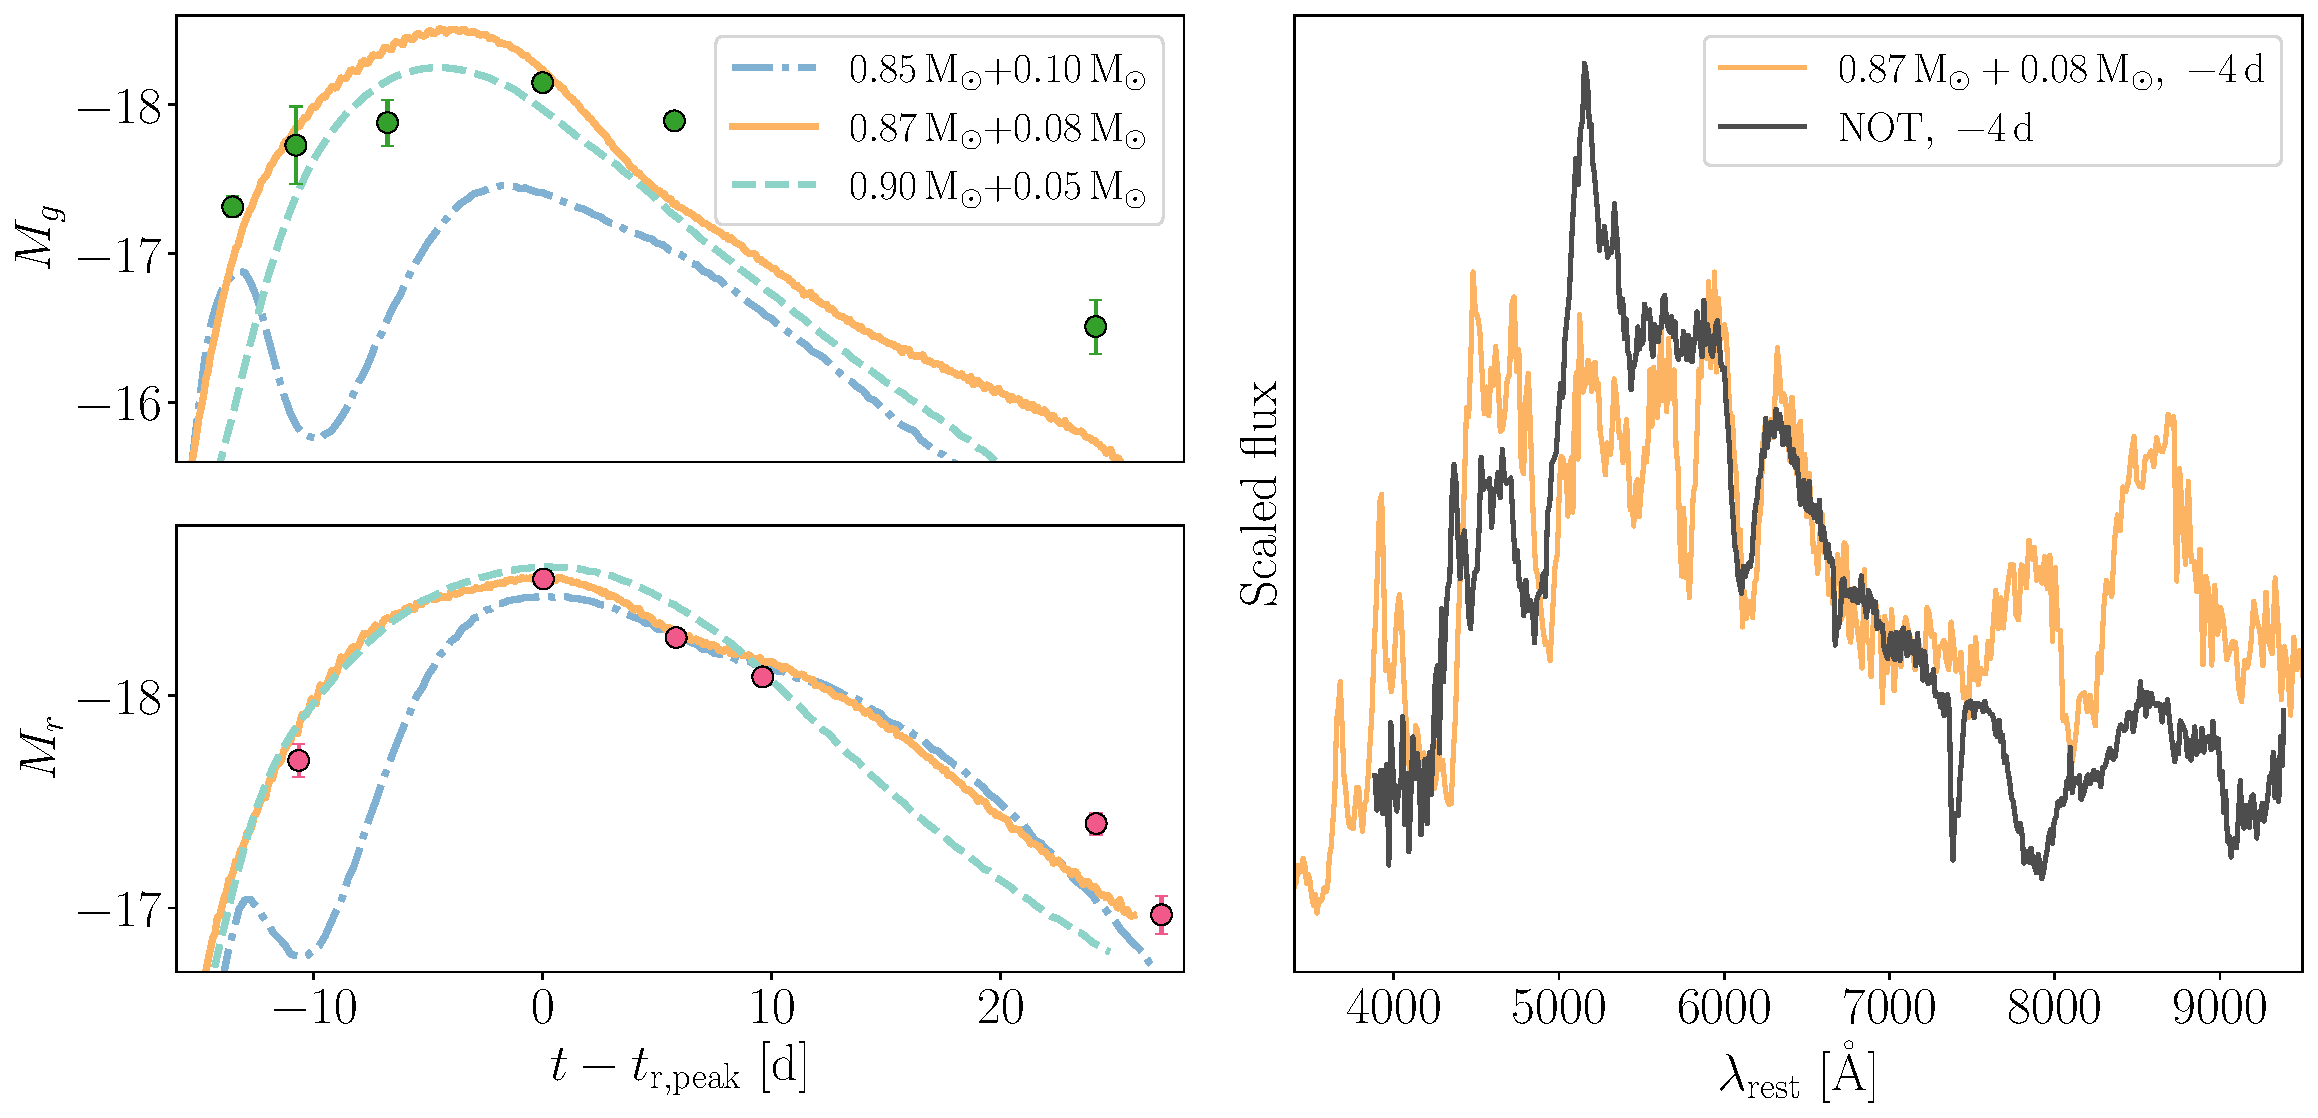
\includegraphics[width=\textwidth]{model.pdf}
    \caption{Spectrophotometric comparison of \sn\ observations with a few He-shell DDet models from \citet{polin_observational_2019}. {\it Left:} Light curve comparison. The model parameters are indicated in the legend as (C/O core mass $+$ He-shell mass). The upper (lower) panel shows the evolution in $r$-band ($g$-band) absolute magnitudes. {\it Right:} Comparison of the observed spectrum with the $0.87\,\mathrm{M_\odot}$ C/O core $+$ $0.08\,\mathrm{M_\odot}$ He-shell model before peak luminosity. Each spectrum is normalized by the median flux between 6500 and 7500\,\AA, and binned with a size of 10\,\AA. The synthetic spectrum 4\,days before the $r$-band peak best matches the ALFOSC spectrum (Galactic extinction corrected), which was obtained $\sim$4\,days before the $r_\mathrm{ZTF}$-band peak. All the phases have been rescaled to the host galaxy rest frame.}
    \label{fig:model}
\end{figure*}

\subsection{The 1\,\micron\ Feature} \label{sec:1um}
\begin{figure}
    \centering
    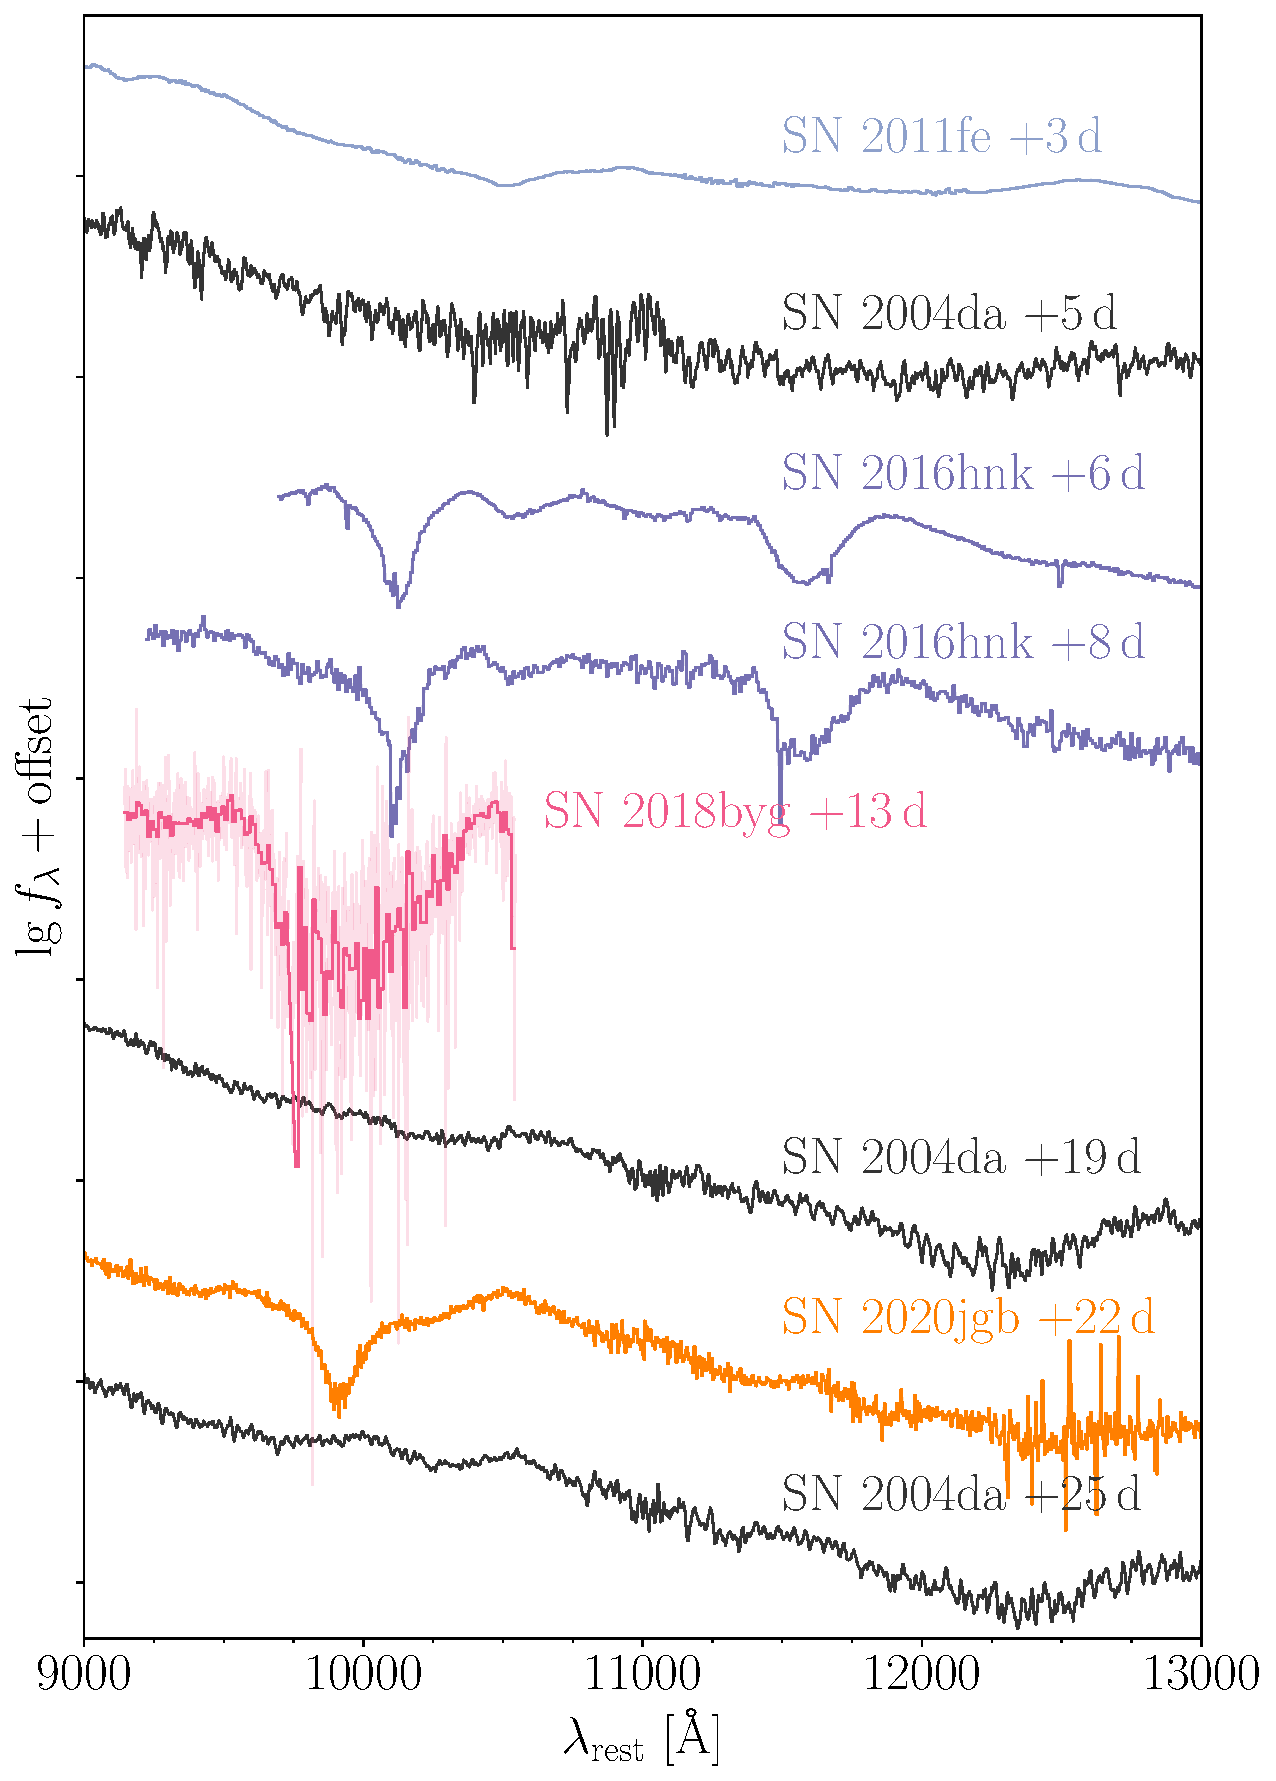
\includegraphics[width=\linewidth]{NIR_spec_comp.pdf}
    \caption{The NIR spectra of normal SNe\,Ia SN\,2011fe \citep{Mazzali_2014} and SN\,2004da \citep{Marion2009_NIR} and three sub-luminous SNe\,Ia  as He-shell DDet candidates, namely SN\,2016hnk \citep{galbany_16hnk_2019}, SN\,2018byg \citep{de_18byg_2019}, and \sn\ (this work). All three He-shell DDet candidates show prominent absorption near 1\,\micron.}
    \label{fig:NIR_comp}
\end{figure}

While the nature of the 1\,\micron\ feature remains uncertain, other He-shell DDet candidates show similar complexity in this region. In the currently small sample, only three objects (SN\,2016hnk, SN\,2018byg, and \sn) have at least one available NIR spectrum (all obtained at different phases), each exhibiting strong absorption features near 1\,\micron, as shown in Figure~\ref{fig:NIR_comp}. SN\,2016hnk has two deep absorption features at $\sim$1.02\,\micron\ and $\sim$1.17\,\micron, both are at a longer wavelength than the 1\,\micron\ feature in \sn. It is suggested in \citet{galbany_16hnk_2019} that both of them are caused by \ion{Fe}{2}, though they are deeper than in other SNe\,Ia. The velocity of the 1.02\,\micron\ feature is $\sim$21,000\,\kms\ assuming a \ion{He}{1} $\lambda$10830 origin, which, just like for \sn, is about the same as the HVFs of the \ion{Ca}{2} IRT (see Figure~\ref{fig:hvf_comp}). The PVFs of the \ion{Ca}{2} IRT of both SNe have a similar expansion velocity of $\sim$10,000\,\kms. Such a consistency in velocities is also seen in SN\,2018byg (see Figure~\ref{fig:hvf_comp}). The large width and low SNR for the 1\,\micron\ feature in SN\,2018byg make it difficult to determine an exact line velocity. The feature may be a mixture of several different lines in SN\,2018byg. 

\citet{Dong_16dsg_2022} recently presented another thick He-shell DDet candidate, SN\,2016dsg, with an absorption line around $\sim$0.97--1.05\,\micron\ in a low-SNR NIR spectrum at $+16.6$\,days\footnote{SN\,2016dsg was discovered on the decline. The phase is relative to the discovery time.}. Assuming a \ion{He}{1} $\lambda$10830 origin, the minimum of the absorption profile (at $\sim$1.03\,\micron, see Figure~4 in \citealp{Dong_16dsg_2022}) corresponds to an expansion velocity of $\sim$15,000\,\kms. Interestingly, SN\,2016dsg shows the least prominent HVFs of \ion{Ca}{2} IRT ($v_\mathrm{SN\,2016dsg} \approx 15$,000\,\kms) among all the He-shell DDet candidates with NIR spectra. Once again, the scenario where both the unburnt helium and the high velocity calcium are located at the outermost shell is favored.

Unfortunately, none of the spectra for SN\,2016dsg, SN\,2016hnk, or SN\,2018byg cover the 2\,\micron\ region, thus it is not possible to identify the presence of helium decisively. But if the 1\,\micron\ feature of these objects are of the same origin, they are more likely to be correlated with the high velocity ejecta lying in the outmost region in the supernovae, because at least for \sn, SN\,2016dsg, and SN\,2016hnk, the difference in their photospheric velocities cannot explain the discrepancy in their line velocities of the 1\,\micron\ feature. Then helium is still a promising candidate to cause strong absorption near 1\,\micron\ for these sub-luminous He-shell DDet SNe\,Ia. 

In conclusion, every thick He-shell DDet candidate with available NIR spectra displays a strong absorption feature near 1\,\micron. This feature is not seen in normal SNe\,Ia. Interestingly, the available NIR spectra are all obtained at different epochs, suggesting this feature may be long lived. If the feature is due to \ion{He}{1}, then DDet explosions exhibit a wide diversity in the expansion velocity. While it remains to be confirmed in a larger sample, we speculate that anomalously strong absorption around 1\,\micron\ is a distinctive attribute of He-shell DDet SNe and that this feature can be used to identify and select events relative to normal SNe\,Ia.

\begin{figure*}
    \centering
    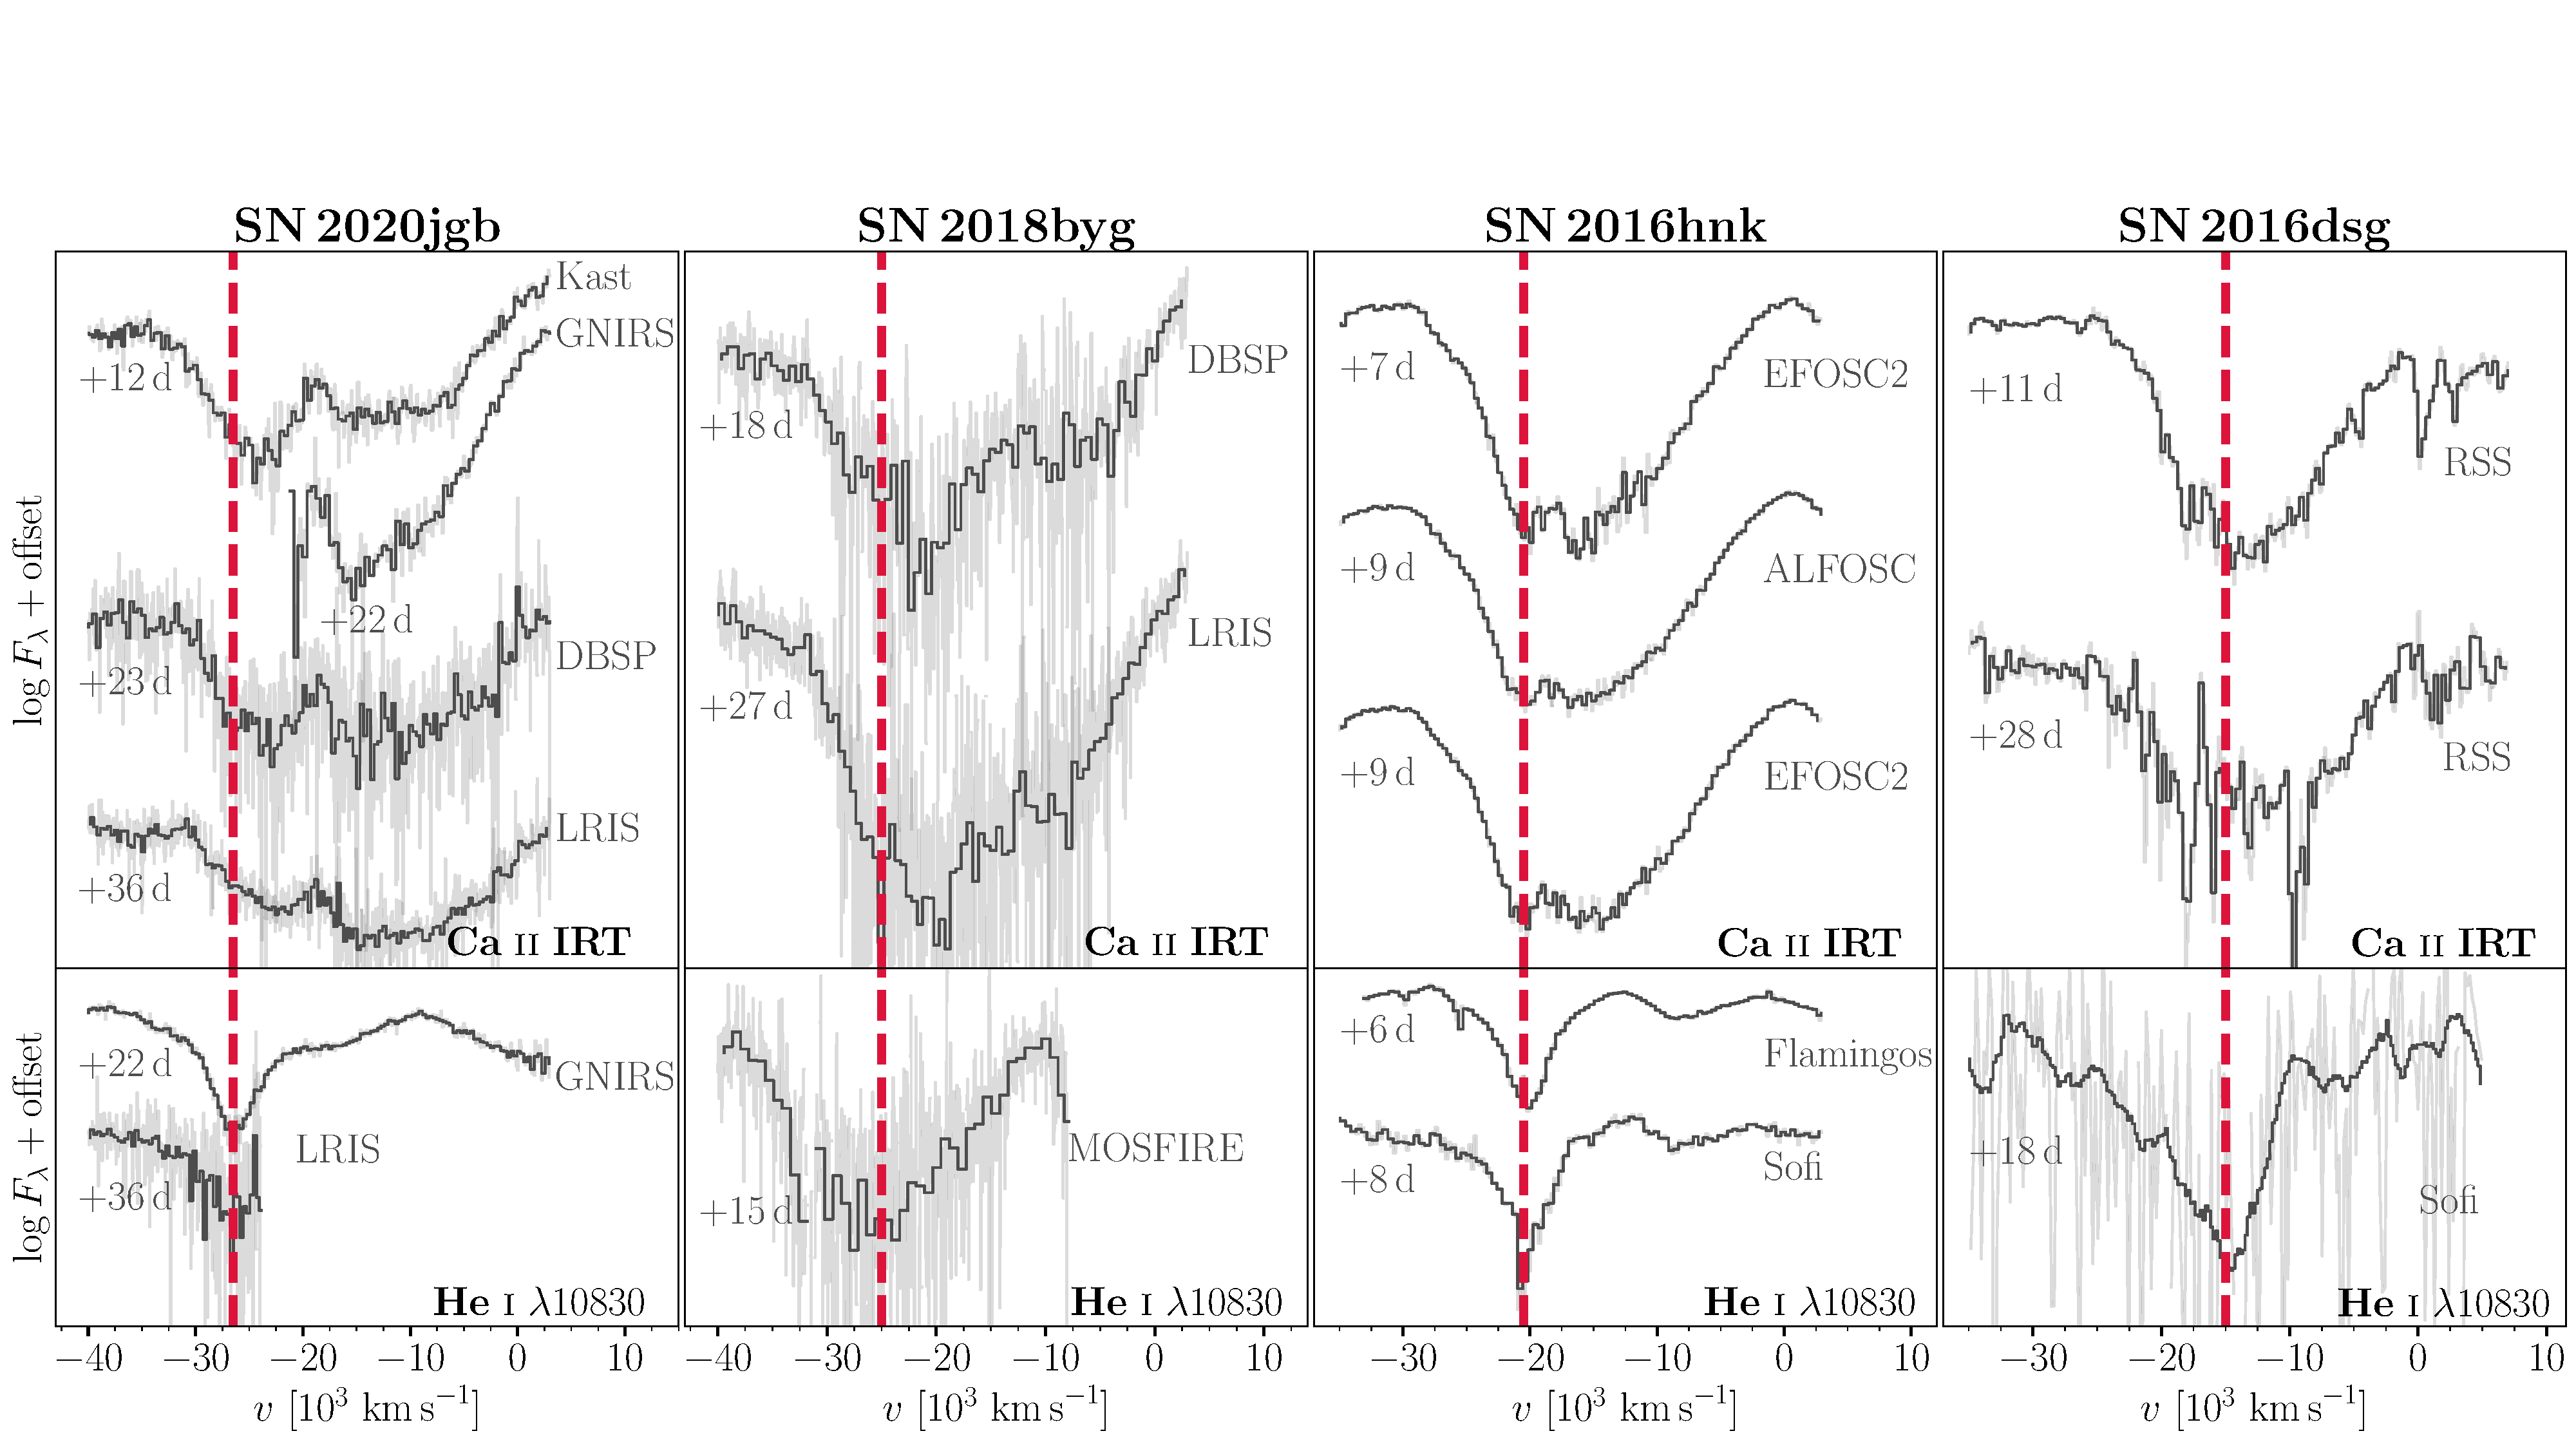
\includegraphics[width=\textwidth]{CaII_HeI_hvf.pdf}
    \caption{Spectra of \sn, SN\,2018byg \citep{de_18byg_2019}, and SN\,2016hnk \citep{galbany_16hnk_2019} in the velocity space, showing the similarity in expansion velocities of the 1\,\micron\ features (lower panels) with the \ion{Ca}{2} IRT absorption features (upper panels), assuming the 1\,\micron\ features are associated with \ion{He}{1} $\lambda$10830. The red dashed lines mark the minimum of each 1\,\micron\ feature, which are displayed to guide the eyes.}
    \label{fig:hvf_comp}
\end{figure*}

\subsection{The Host Environment of He-shell DDet SNe} \label{sec:host}

\begin{figure*}
    \centering
    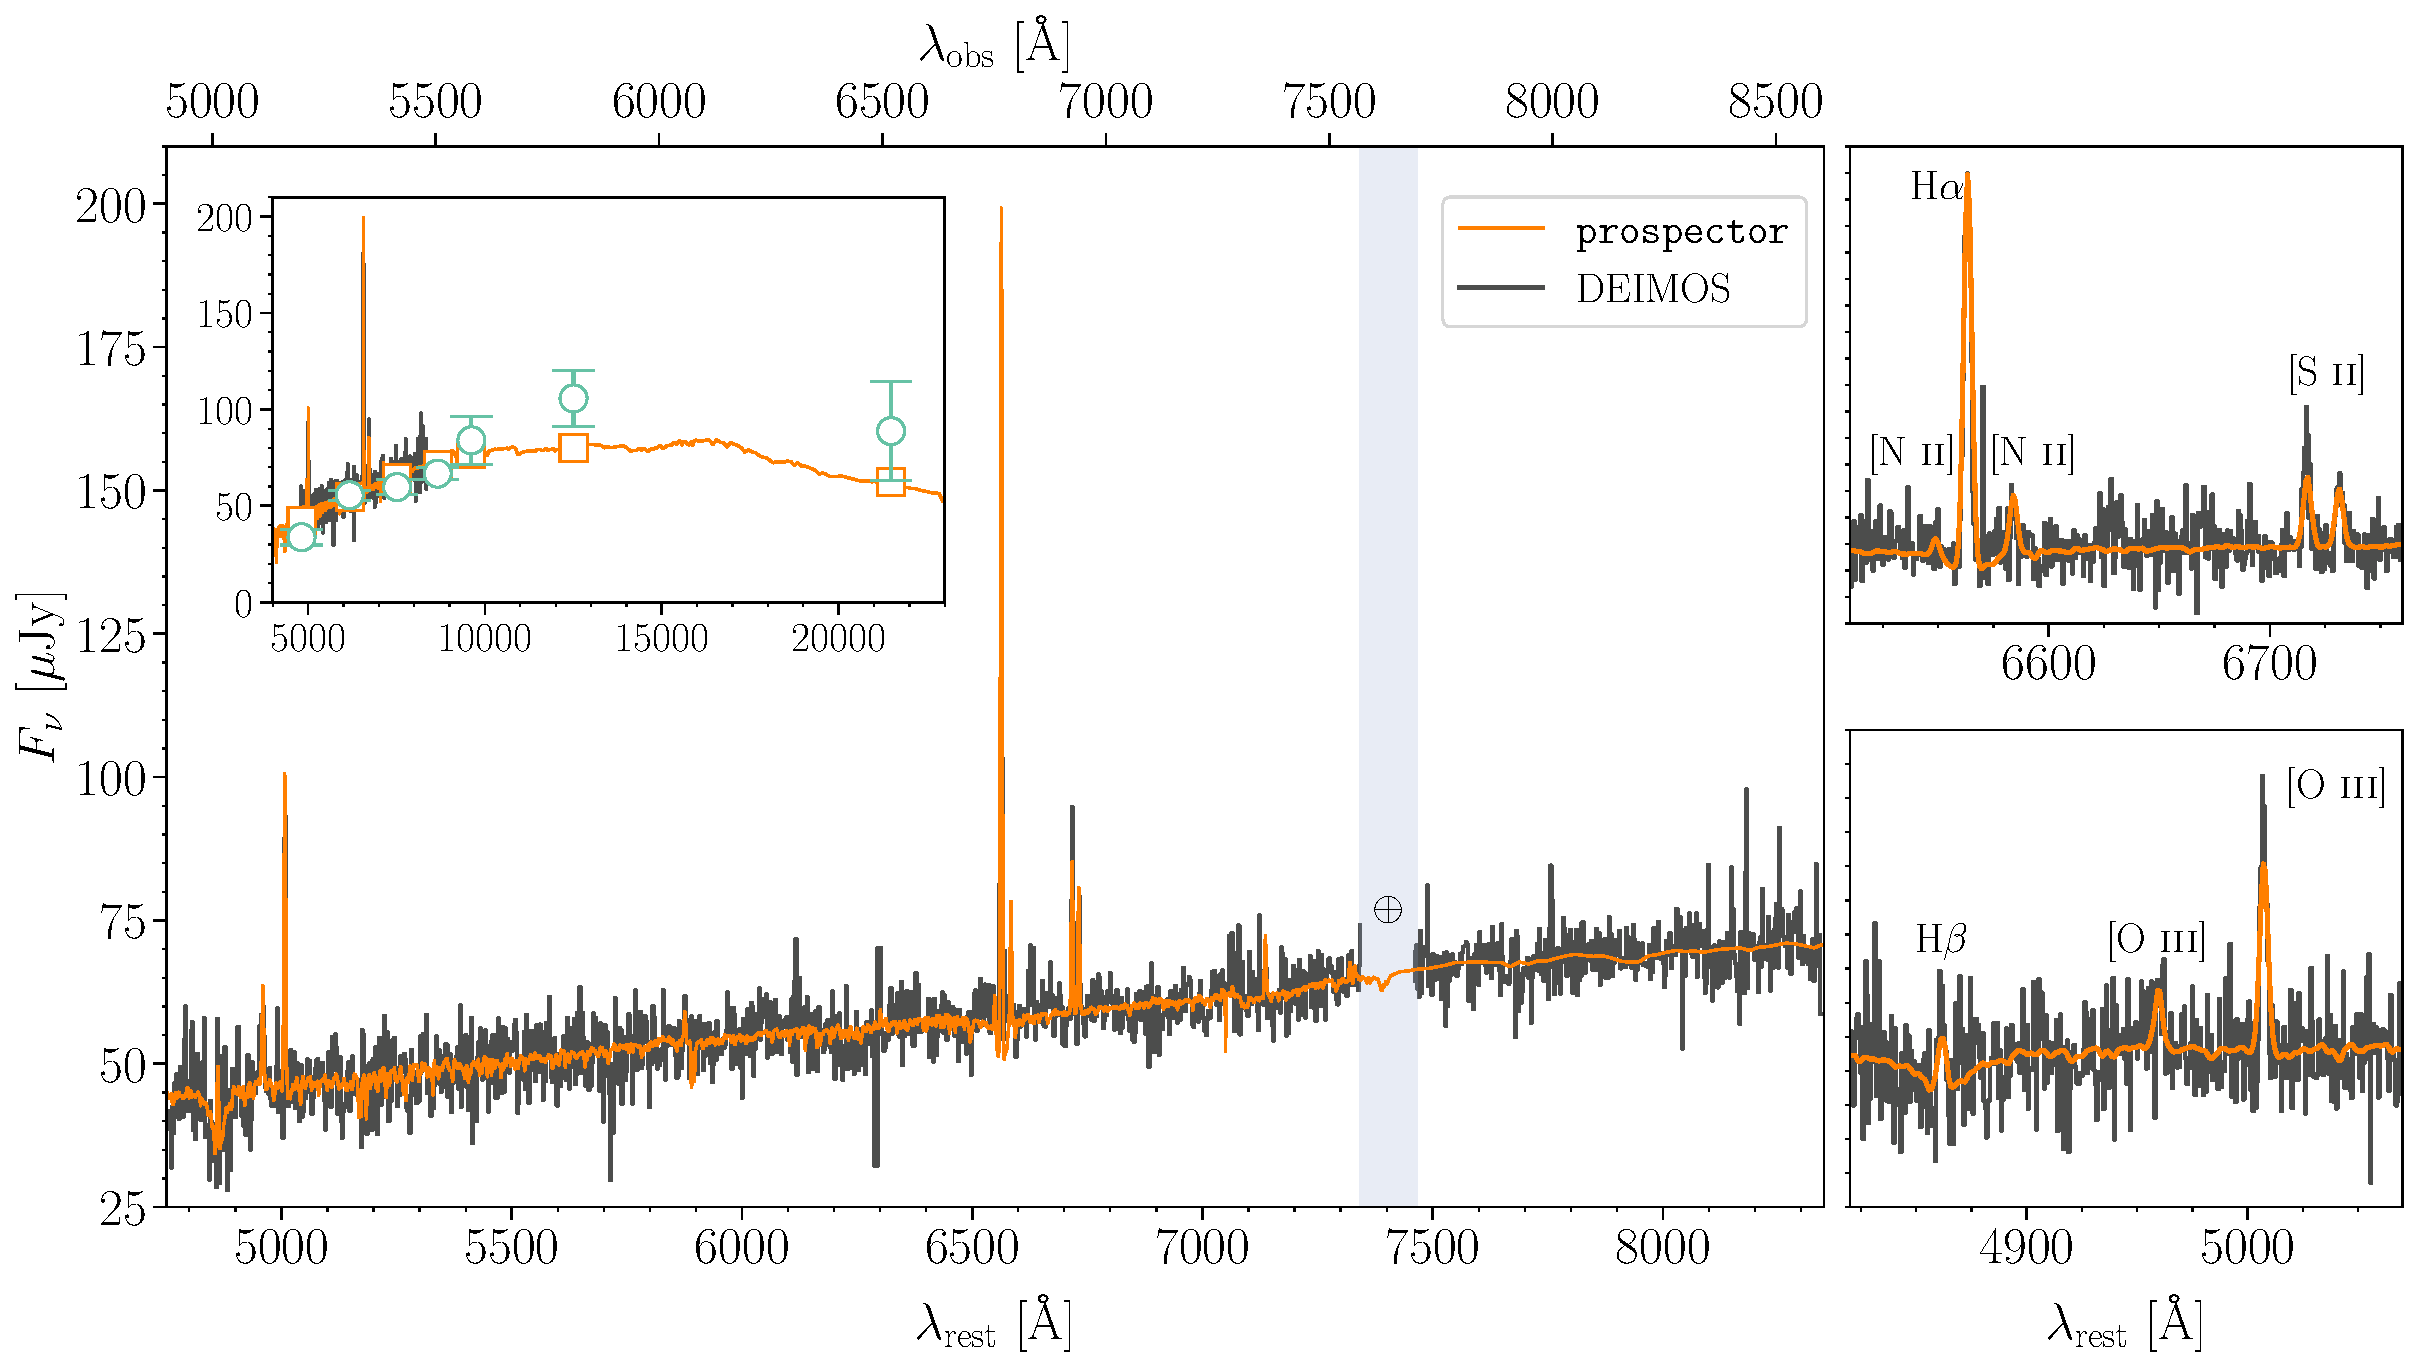
\includegraphics[width=\textwidth]{DEIMOS_20jgb.pdf}
    \caption{The spectral energy distribution (SED) of the star-forming dwarf galaxy PSO J175312.663+005122.078, the host galaxy of \sn, and the model from \texttt{prospector}. When fitting the SED with \texttt{prospector}, the DEIMOS spectrum is automatically rescaled to fit the archival photometry from the Panoramic Survey Telescope and Rapid Response System \citep[Pan-STARRS;][{\it g, r, i, z, y} Kron magnitudes]{PS1_2016}  and the VISTA Hemisphere Survey \citep[VHS;][J and $\mathrm{K}_\mathrm{s}$ Petrosian magnitudes]{VHS_2013}. {\it Left:} the SED in the optical band (4750-8350\,\AA\ in the rest frame of the host galaxy). The black line corresponds to the observed spectrum, binned with a size of 2\,\AA. The orange line is the \texttt{prospector} model produced from the median of the stellar population property posterior distributions. The blue shaded region is masked in the fitting due to the strong telluric lines. {\it Inner panel:} the same comparison, but covers $g$-band through $\mathrm{K_s}$-band (4000-24000\,\AA). Apart from the spectra, we also show the multi-band photometry (green circles) and the best-fit magnitudes (orange squares). {\it Right:} spectra around the most prominent emission lines. {\it Top right:} H$\alpha$, [\ion{N}{2}] $\lambda\lambda$6548, 6583, [\ion{S}{2}] $\lambda\lambda$6716, 6731. {\it Bottom right:} H$\beta$, [\ion{O}{3}] $\lambda\lambda$4959, 5007.}
    \label{fig:host_spec}
\end{figure*}

We model the host galaxy of \sn\ using \texttt{prospector} \citep{Johnson_prospector_2021}, a package for principled inference of stellar population properties using photometric and/or spectroscopic data. Prospector applies a nested sampling fitting routine through \texttt{dynesty} \citep{Speagle_dynesty_2020} to the observed data and produces posterior distributions of the stellar population properties and model spectral energy distributions (SEDs) with use of \texttt{Python-FSPS} \citep{Conroy_2009,Conroy_2010}. Our observed data include the Galactic extinction corrected DEIMOS spectrum, as well as the archival photometric data from the Panoramic Survey Telescope and Rapid Response System \citep[Pan-STARRS;][{\it g, r, i, z, y} Kron magnitudes]{PS1_2016}  and the VISTA Hemisphere Survey \citep[VHS;][J and $\mathrm{K}_\mathrm{s}$ Petrosian magnitudes]{VHS_2013}. We use a parametric delayed-$\tau$ star formation history, given by Equation~(1) in \citet{Nugent_2020} and defined by the e-folding factor $\tau$, the Galactic dust extinction law \citep{Cardelli_1989}, and Chabrier initial mass function \citep{Chabrier_2003} to the model. We further apply a mass-metallicity relation \citep{Gallazzi_2005} to sample realistic stellar masses and metallicities and a dust law that ensures young stellar light attenuates dust twice the amount of old stellar light, as has been observed.  We also add a nebular emission model with the gas-phase metallcity and a gas ionization parameter to correctly measure the strength of the emission lines in the DEIMOS spectrum. The model spectral continuum is built from a 10th order Chebyshev polynomial. We determine the stellar mass and star-formation rate (SFR) from the \texttt{prospector} output, as shown in \citet{Nugent_2022}. The estimated stellar mass is $\log (M_*\,[\mathrm{M_\odot}])=7.79_{-0.06}^{+0.07}$, and the specific star-formation rate (sSFR) is $\log (\mathrm{sSFR}\,[\mathrm{yr}^{-1}])=-10.25_{-0.08}^{+0.09}$, with the uncertainties denoting the 68\% highest posterior density regions.

In Figure~\ref{fig:host}, we show the sSFR and the stellar mass for the host galaxies of six He-shell DDet candidates. Again using \texttt{prospector}, we fit the stellar properties for all the other candidates with optical spectra from the Sloan Digital Sky Survey \citep[SDSS;][]{York_2000} and photometry from the DESI Legacy Imaging Surveys \citep[][{\it g, r, z, $W_1$, $W_2$, $W_3$, $W_4$} magnitudes]{Dey_2019}. With mid-infrared (MIR) photometry available, \texttt{prospector} can better estimate the overall dust extinction in the host galaxy and the contribution of an active galactic nucleus (AGN) to the SED. We therefore add two additional parameters to our prospector fit to sample the MIR optical depth and fraction of AGN luminosity. Unfortunately, two hosts (those of SN\,2016hnk and SN\,2019ofm) are nearby ($z\lesssim 0.03$) late-type galaxies with extended, spatially resolved spiral structures. Examination of the photometry model from Legacy Surveys (LS) shows that the galaxy aperture does not include the blue, diffuse star-forming regions of these galaxies. Fitting the SDSS spectra + LS photometry would inevitably underestimate their sSFR. For the host of SN\,2016hnk, we instead adopt the results in \citet{Dong_Ca-rich_2022}, which uses broadband far-ultraviolet (FUV) to far-infrared (FIR) photometry from the $z=0$ Multiwavelength Galaxy Synthesis I \citep[z0MGS;][]{Leroy_2019} to characterize the stellar population with \texttt{prospector}. For the host of SN\,2019ofm, there are no archival stellar population data available, so we still show our best-fit parameters in Figure~\ref{fig:host}, with the caveat that the sSFR should be regarded as a lower limit. In addition, the host of SN\,2018aoz (NGC\,3923) is a local ($z=0.00580$) early-type galaxy and is outside the SDSS footprint, so we adopt its stellar population properties from the Census of the Local Universe (CLU) catalog \citep{de_Ca_rich_2020}. PTF\,09dav is not displayed in Figure~\ref{fig:host} because it appears to be hostless, with the nearest galaxy with a known redshift being a star-forming late-type galaxy $\sim$40\,kpc away \citep{Sullivan_2011}. Nonetheless, it is close to several extended sources with low surface brightness, which could be faint dwarf galaxies \citep[see Figure 3 in][]{Kasliwal_2012}. Its nebular phase spectrum shows H$\alpha$, which indicates potential star-formation, but could also be explained with photoionized gas around the transient \citep{Kasliwal_2012}.

Figure~\ref{fig:host} reveals that DDet SNe emerge in both star-forming and passive galaxies, which is true for both thin He-shell objects of normal luminosity (SN\,2016jhr in a star-forming host; SN\,2018aoz in a passive host) and thick He-shell, sub-luminous objects (SN\,2020jgb in a star-forming host; SN\,2018byg in a passive host). Their locations in host galaxies also show large variety. SN\,2020jgb has a small projected physical offset ($\sim$0.2\,kpc) to the center of its host, a star-forming dwarf galaxy, so it is likely to originate from a young, star-forming environment. SN\,2016hnk has a moderate projected host offset ($\sim$4\,kpc) and a potential origin in an \ion{H}{2} region with ongoing star-formation \citep{galbany_16hnk_2019}. SN\,2019ofm has a large projected offset ($\sim$11\,kpc) but is still on the blue, diffuse spiral arm, as shown in its DECaLS image \citep{Dey_2019}. Other objects, including the recently reported SN\,2016dsg and OGLE-2013-SN-079 \citep{Dong_16dsg_2022}, show large projected host offsets ($\gtrsim$10\,kpc) and lie in the galaxy outskirts, which usually indicates origin in old stellar population. %\chang{no reference to 18byg offset here?} \adam{I did the calculation myself with Astropy.}

In this sense, the He-shell DDet sample resembles the normal SN\,Ia population, which can occur in both star-forming and quenched galaxies \citep[e.g.,][]{Sullivan_2006, Smith_2012}, and is very different from some other types of thermonuclear supernovae, such as Type-Iax supernovae (SNe\,Iax) which almost only appear in star-forming galaxies, or 91bg-like and 02es-like objects, which prefer old stellar environments \citep[see the review in][]{Jha_2019}. This favors the postulated sequence that He-shell DDet SNe may make up a substantial fraction of the normal SNe\,Ia, which is supported by stellar metallicity observations \citep{Sanders_2021, Eitner_2022}.

The diversities in host environments indicate multiple formation channels in the He-shell DDet SN population. Those in the star-forming environments, \sn\ being the most unambiguous example, could originate from some analogues of the two subdwarf B binaries with WD companions \citep{Geier_2013, Kupfer_2022} discovered in young stellar populations.
On the other hand, those with large host offsets could not be easily formed {\it in situ}. Similarly, many Ca-rich transients are also observed in remote locations \citep{Lunnan_2017}, for which some dynamical formation channels have been proposed. To reach the outskirts of galaxies, WD binaries would need to be ejected by globular clusters \citep{Shen_2019} or supermassive black holes \citep{Foley_2015} before explosions. Given that some Ca-rich transients show characteristic DDet properties \citep{de_Ca_rich_2020}, these channels may also be applicable to some of the He-shell DDet SNe. 

The robust detection of \sn\ in a star-forming region also agrees with independent studies on SN\,Ia progenitors using stellar metallicity observations. After measuring the manganese abundance in the Sculptor dwarf spheroidal galaxy, it is argued in \citet{de_los_reyes_manganese_2020} that sub-\Mch\ SNe\,Ia dominate the chemical evolution of a galaxy, while near-\Mch\ SNe tend to take over at later times. This indicates that observationally, sub-\Mch\ SNe\,Ia might have a stronger preference towards younger stellar populations than near-\Mch\ SNe\,Ia. %\chang{Isn't this also the conclusion of the Eitner paper?} \adam{The Eitner paper didn't talk about how the ignition mechanisms are related to the stellar population.} 
Since He-shell DDet is one of the most favored channel to ignite a sub-\Mch\ WD, we would expect the majority of SNe\,Ia in star-forming galaxies (at least the dwarfs) would undergo He-shell DDet. We note that while \sn\ is the first confirmed He-shell DDet SN in a star-forming dwarf, which indicates that thick He-shell DDet SNe might be intrinsically rare, the same may not be true for those ignited by a thin He-shell since they would look just as  `normal' a few days after explosion \citep{Ni_2022}. Unfortunately, few SNe\,Ia are observed in such an early phase to date (SN\,2016jhr and SN\,2018aoz being two of them), thus we might have missed a great number of thin He-shell DDet SNe. A systematic study based on prompt follow-up observations on the infant SNe\,Ia will help verify this implication, with more efficient time domain surveys in the future.

\begin{figure}
    \centering
    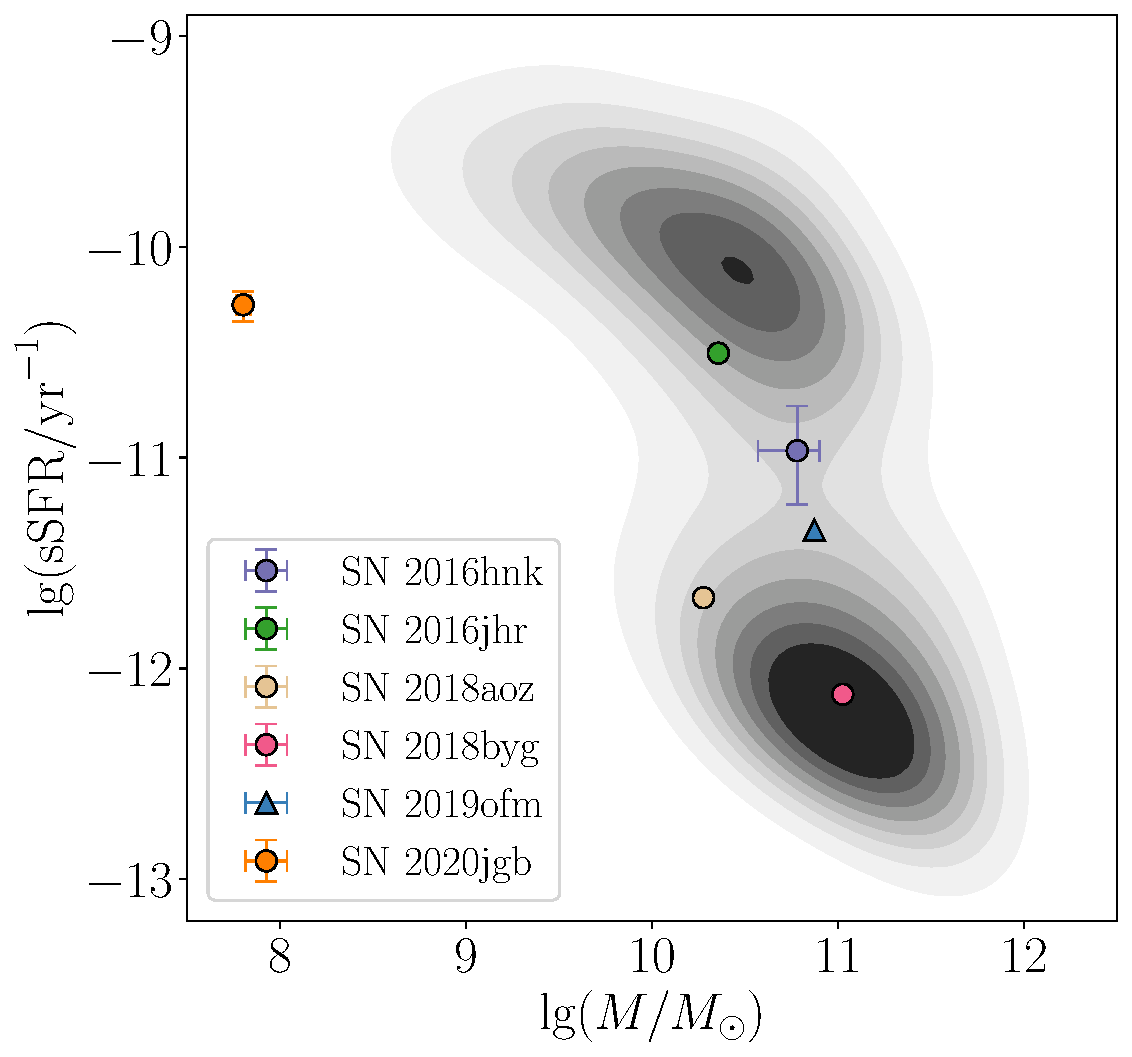
\includegraphics[width=\linewidth]{host.pdf}
    \caption{The specific star-formation rate (sSFR) and the stellar mass for the host galaxies of He-shell DDet candidates, showing He-shell DDet SNe could emerge in both star-forming and passive galaxies. The properties for the hosts of SN\,2016hnk and SN\,2018aoz are taken from \citet{Dong_Ca-rich_2022} and the CLU catalog \citep{de_Ca_rich_2020}, respectively. For the sSFR in the host of SN\,2019ofm, only a lower limit is shown (the circle with an arrow). The grey contours correspond to the bivariate distributions of stellar mass and sSFR for galaxies in the SDSS MPA-JHU DR8 catalog \citep{Kauffmann_SDSS_2003,Brinchmann_SDSS_2004}, visualized using kernel density estimation (KDE) with the data visualization library \texttt{seaborn} \citep{Waskom_seaborn_2021}. Galaxies with BPT classification as AGNs or LINERs are excluded, since certain spectral features (e.g., H$\alpha$ emission) due to nuclear activities might be misinterpreted as star formation.}
    \label{fig:host}
\end{figure}

\section{Conclusions} \label{sec:conclusion}
We have presented observations of \sn, a peculiar SN\,Ia. It has a low luminosity, red $g_\mathrm{ZTF}-r_\mathrm{ZTF}$ colors, and strong line-blanketing in the optical spectra near maximum light, all of which are highly similar to SN\,2018byg \citep{de_18byg_2019}, whose observational properties could be explained by the detonation of a shell of helium on a sub-\Mch WD. Fitting the light curves of \sn\ to a grid of models from \citet{polin_observational_2019}, we show a $\sim$0.87\,$\mathrm{M_\odot}$ WD beneath a $\sim$0.08\,$\mathrm{M_\odot}$ He-shell provides a reasonable match to the observed spectrophotometric evolution of \sn.

A high-SNR NIR spectrum obtained three weeks after maximum light shows a prominent absorption feature near 1\,\micron, which could be produced by the unburnt helium (\ion{He}{1} $\lambda$10830) in the outermost ejecta expanding at a high velocity ($\sim$26,000\,\kms). At the same epoch, the \ion{Ca}{2} IRT also exhibits similarly high velocities ($\sim$24,000\,\kms). To date only four candidate He-shell DDet SNe have observed NIR spectra. Interestingly, all of them show deep absorption features near 1\,\micron, which, if assumed to be \ion{He}{1} $\lambda$10830, would be expanding at a very similar velocity to the HVFs of \ion{Ca}{2} IRT. For these candidates the \ion{Ca}{2} HVFs and putative \ion{He}{1} velocities show significant diversity ranging from $\sim$15,000\,\kms\ in SN\,2016dsg to $\sim$24,000\,\kms\ in \sn. If it is the unburnt helium and the newly synthesized calcium from the He-shell that produce these line features, such a consistency in the expansion rates of different absorption lines would be naturally explained. However, we could not find unambiguous evidence for other \ion{He}{1} absorption features, such as \ion{He}{1} $\lambda$20581, so we cannot claim a definitive detection of helium in \sn. Nonetheless, alternative possibilities (\ion{Mg}{2}, \ion{C}{1}, \ion{Fe}{2}) that may cause the 1\,\micron\ feature are deemed even less likely. Helium is thus the most plausible explanation for the apparently ubiquitous 1\,\micron\ features.

We propose that He-shell DDet SNe can be robustly identified with NIR spectra. For transients showing a clear 1\,\micron\ feature, to test its potential association with \ion{He}{1} $\lambda$10830 one could follow the checklist below.
\begin{itemize}
    \item Search for \ion{He}{1} $\lambda$20581. A caveat is that one should not always expect to see significant \ion{He}{1} $\lambda$20581 absorption in He-shell DDet SNe, since this line is weaker than \ion{He}{1} $\lambda$10830 and could be almost invisible when the He-shell is thin \citep{Boyle2017_Helium}. The strong telluric lines near 2\,\micron\ also add to the difficulty in detecting \ion{He}{1} $\lambda$20581.
    \item Calculate the line velocity assuming an origin in \ion{He}{1} $\lambda$10830 and check if it is comparable with the HVFs velocity in the \ion{Ca}{2} IRT absorption at a similar phase. While both the detonation recipe in a He-shell DDet model and the viewing angles would affect the observed \ion{He}{1}/\ion{Ca}{2} velocity, we still expect the elements along the line-of-sight to expand at a similar velocity, if they all have a He-shell origin.
    \item Exclude the possibility of other strong lines. If the NIR spectrum is obtained before the peak of the SN, strong \ion{Mg}{2} and \ion{C}{1} absorption \citep{Hsiao_CSP_2019} would be possible contaminants. Otherwise if the 1\,\micron\ feature is seen in the transitional-phase spectrum when the inner region of the SN becomes visible, we need to carefully rule out the possibility of \ion{Fe}{2} origin \citep{Marion2009_NIR}.
\end{itemize}
   %\chang{I think this can be cleaned up a bit - think about this as bullet points, what is the most direct way to describe these steps?}

The He-shell DDet SNe in the tiny sample show diversities in various observational properties, including the peak luminosity, color evolution, chemical abundances and line velocities, which could be explained by a large variety of He-shell and WD masses \citep{polin_observational_2019,Shen_2D_2021}, viewing angles \citep{Shen_2D_2021}, and the initial chemical compositions in He-shell \citep{Kromer_DD_2010}. In addition, they are discovered in both old and young stellar populations, \sn\ being the first unambiguous thick He-shell DDet candidate in a star-forming galaxy. If, as has been argued \citep[e.g.,][]{Sanders_2021, Eitner_2022}, a substantial fraction of normal SNe\,Ia are triggered by He-shell DDet, then we would naturally expect He-shell DDet SNe to emerge in both star-forming and passive galaxies as normal SNe\,Ia do \citep[e.g.,][]{Sullivan_2006,Smith_2012}, which is exactly what we observe. This is unlike some other subtypes of SNe\,Ia \citep{Jha_2019} which strongly prefer either star-forming galaxies (e.g., SNe\,Iax) or passive galaxies (e.g., 91bg-like and 02es-like objects). Nonetheless, it remains to be examined whether thick He-shell DDet SNe stem from similar progenitors as the majority of normal SNe\,Ia, or if their massive He-shells could only be developed in a completely distinctive population of binary systems.

\begin{acknowledgements}
    The authors are thankful to Eddie Schlafly and Dustin Lang for suggesting photometry from DESI Legacy Imaging Surveys in SED fitting.

    \adam{Other people to acknowledge + Fundings + Collaborators to add their fundings}

    This work is based on observations obtained with the Samuel Oschin Telescope 48-inch and the 60-inch Telescope at the Palomar Observatory as part of the Zwicky Transient Facility project. ZTF is supported by the National Science Foundation under Grant No. AST-1440341 and a collaboration including Caltech, IPAC, the Weizmann Institute of Science, the Oskar Klein Center at Stockholm University, the University of Maryland, the University of Washington, Deutsches Elektronen-Synchrotron and Humboldt University, Los Alamos National Laboratories, the TANGO Consortium of Taiwan, the University of Wisconsin at Milwaukee, and Lawrence Berkeley National Laboratories. Operations are conducted by COO, IPAC, and UW. SED Machine is based upon work supported by the National Science Foundation under Grant No. 1106171. This work is also based on observations made with the Nordic Optical Telescope, owned in collaboration by the University of Turku and Aarhus University, and operated jointly by Aarhus University, the University of Turku and the University of Oslo, representing Denmark, Finland and Norway, the University of Iceland and Stockholm University at the Observatorio del Roque de los Muchachos, La Palma, Spain, of the Instituto de Astrofisica de Canarias.
\end{acknowledgements}

\facility{PO:1.2m (ZTF), PO:1.5m (SEDM), Gemini:Gillett (GNIRS), Hale (DBSP), NOT (ALFOSC), Shane (Kast Double spectrograph), Keck:I (LRIS), Keck:II (DEIMOS).}

\software{\texttt{astropy} \citep{Astropy_2013, Astropy_2018}, \texttt{CASTRO} \citep{Almgren_Castro_2010}, \texttt{dynesty} \citep{Speagle_dynesty_2020}, \texttt{emcee} \citep{emcee_2013}, \texttt{matplotlib} \citep{Matplotlib_2007}, \texttt{prospector} \citep{Johnson_prospector_2021}, \texttt{PypeIt} \citep{pypeit:zenodo}, \texttt{pysedm} \citep{Rigault_pysedm_2019}, \texttt{Python-FSPS} \citep{Conroy_2009,Conroy_2010} \texttt{scipy} \citep{Scipy_2020}, \texttt{seaborn} \citep{Waskom_seaborn_2021}, \texttt{SEDONA} \citep{Kasen_Sedona_2006}.}

\bibliography{SN2020jgb, software}
\bibliographystyle{aasjournal}

%% This command is needed to show the entire author+affiliation list when
%% the collaboration and author truncation commands are used.  It has to
%% go at the end of the manuscript.
%\allauthors

%% Include this line if you are using the \added, \replaced, \deleted
%% commands to see a summary list of all changes at the end of the article.
%\listofchanges

\end{document}

% End of file `sample631.tex'.